%
\documentclass{report}
\usepackage{amsmath}
\usepackage{amssymb}
\usepackage{amsthm}
\usepackage{amscd}
\usepackage{fullpage}
\usepackage{braket}
\usepackage{dsfont}
\usepackage{mdframed}
\usepackage{slashed}
\usepackage{comment}
\usepackage{feynmf}
\usepackage[usenames,dvipsnames,svgnames,table]{xcolor}
\usepackage{tikz}
\usetikzlibrary{positioning}

\theoremstyle{plain}
\newtheorem{theorem}{Theorem}[section]
\newtheorem{lemma}[theorem]{Lemma}
\newtheorem{proposition}[theorem]{Proposition}
\newtheorem{corollary}[theorem]{Corollary}

\theoremstyle{definition}
\newtheorem{definition}[theorem]{Definition}
\newtheorem{axiom}{Axiom}
\newtheorem{example}[theorem]{Example}
\newtheorem{exercise}{Exercise}[section]

\theoremstyle{remark}
\newtheorem*{remark}{Remark}
\newtheorem*{note}{Note}

\newcommand{\FR}[2]{\frac{#1}{#2}}
\newcommand{\PFR}[2]{\left(\frac{#1}{#2}\right)}
\newcommand{\SFR}[2]{\sqrt{\frac{#1}{#2}}}

\newcommand{\mc}{\mathcal}
\newcommand{\lam}{\lambda}
\newcommand{\vphi}{\varphi}
\newcommand{\om}{\omega}
\newcommand{\Om}{\Omega}
\newcommand{\gam}{\gamma}
\newcommand{\sg}{\sigma}
\newcommand{\di}{\partial}
\newcommand{\sdi}{\slashed\partial}
\newcommand{\ddi}[2]{\FR{\partial {#1}}{\partial {#2}}}
\newcommand{\hp}{\hat p}
\newcommand{\ha} { a}
\newcommand{\hb} { b}
\newcommand{\hbd} { b^\dagger}
\newcommand{\had}{ a^\dagger}
\newcommand{\iden}{\mathds{1}}
\newcommand{\colr}[1]{ {\color{red} #1 } }
\newcommand{\colb}[1]{ {\color{blue} #1 } }
\newcommand{\colf}[1]{ {\color{Fuchsia} #1 } }

\newcommand{\elaborate}{{\color{blue} \textbf{Elaborate.}}}
\newcommand{\CHECK}{{\color{blue} \textbf{CHECK}}}

\DeclareMathOperator{\bC}{\mathbb{C}}
\DeclareMathOperator{\bR}{\mathbb{R}}
\DeclareMathOperator{\bP}{\mathbb{P}}
\DeclareMathOperator{\bN}{\mathbb{N}}
\DeclareMathOperator{\bZ}{\mathbb{Z}}
\DeclareMathOperator{\cA}{\mathcal{A}}
\DeclareMathOperator{\cB}{\mathcal{B}}
\DeclareMathOperator{\cC}{\mathcal{C}}
\DeclareMathOperator{\cD}{\mathcal{D}}
\DeclareMathOperator{\cF}{\mathcal{F}}
\DeclareMathOperator{\cH}{\mathcal{H}}
\DeclareMathOperator{\cI}{\mathcal{I}}
\DeclareMathOperator{\cJ}{\mathcal{J}}
\DeclareMathOperator{\cL}{\mathcal{L}}
\DeclareMathOperator{\cM}{\mathcal{M}}
\DeclareMathOperator{\fg}{\mathfrak{g}}
\DeclareMathOperator{\id}{id}
\DeclareMathOperator{\im}{Im}
\DeclareMathOperator{\re}{Re}
\DeclareMathOperator{\Ad}{Ad}
\DeclareMathOperator{\Sp}{Sp}
\DeclareMathOperator{\SO}{SO}
\DeclareMathOperator{\GL}{GL}
\DeclareMathOperator{\Hom}{Hom}
\DeclareMathOperator{\Aut}{Aut}
\DeclareMathOperator{\so}{so}

\begingroup
    \makeatletter
    \@for\theoremstyle:=definition,remark,plain\do{%
        \expandafter\g@addto@macro\csname th@\theoremstyle\endcsname{%
            \addtolength\thm@preskip\parskip
            }%
        }
\endgroup

\edef\restoreparindent{\parindent=\the\parindent\relax}
\usepackage{parskip}
\restoreparindent

\tikzset{
  particle/.style={thick,draw=black},
  gluon/.style={decorate,draw=black,decoration={coil,aspect=0}},
  vertex/.style={shape=circle,scale=0.3,fill=black,draw=black},
  every loop/.style={thick,draw=black},
  loop left/.style={in=140,out=220,min distance=2cm},
  loop right/.style={in=-40,out=40,min distance=2cm},
  loop above/.style={in=60,out=120,min distance=2.4cm},
  loop below/.style={in=-120,out=-60,min distance=2.4cm}
}

% Macros for "contractions", by Dan Schroeder
% These are a total kludge--use at your own risk!

\newif\ifContLineOne
\newif\ifContLineTwo
\newif\ifContLineThree

% Macro to draw horizontal lines, continuing all contractions in progress.
% Parameter is the symbols to go underneath.  Lines have width .4pt and 
% are separated by 3.2pt of space.  Bottom of lowest line is 14pt above baseline.
\def\conC#1{\vbox{\ialign{##\crcr
  \ifContLineThree\hrulefill\else\vphantom{\hrulefill}\fi\crcr
  \noalign{\kern3.2pt\nointerlineskip}
  \ifContLineTwo\hrulefill\else\vphantom{\hrulefill}\fi\crcr
  \noalign{\kern3.2pt\nointerlineskip}
  \ifContLineOne\hrulefill\else\vphantom{\hrulefill}\fi\crcr
  \noalign{\nointerlineskip}
  $\hfil\textstyle{\vbox to 14pt{}#1}\hfil$\crcr}}}

% Internal macro to draw vertical legs.  dimen2 is height of
% bottom of leg.  The initial value of dimen3+(#2*dimen4) is height
% of top of leg, and must be adjusted if these macros are used under
% different vertical spacing conditions.
\def\DrawLeg#1#2{
  \kern-.2pt              % back up half width of leg
  \dimen2 =#1             % =height of whatever is underneath leg
  \advance\dimen2 by 2pt  % 2pt space below bottom of leg
  \dimen3 = 10.6pt        % base value of height of top of leg
  \dimen4 =3.6pt          % add this much time 1 2 or 3 to base value
  \advance\dimen3 by -\dimen2 
  \multiply\dimen4 by #2
  \advance\dimen3 by \dimen4
  \raise\dimen2 \hbox{\vrule height\dimen3 width .4pt} % draw it
  \kern-.2pt}             % and back up half width of line

% Macro to begin a new contraction.  First parameter is height or level
% (1, 2, or 3); second parameter is the symbol(s) to go underneath
\def\begC#1#2{\setbox0 =\hbox{$\textstyle{#2}$}
  \dimen0=.5\wd0 \dimen1=\ht0
  \conC{\hskip\dimen0}
  \count255=#1
  \ifnum\count255 =1 \ContLineOnetrue\else
  \ifnum\count255 =2 \ContLineTwotrue\else
  \ifnum\count255 =3 \ContLineThreetrue\fi\fi\fi
  \DrawLeg{\dimen1}{\count255}
  \conC{\hskip\dimen0}
  \kern-\dimen0\kern-\dimen0 \box0}

% Macro to end a contraction; same parameters as \begC.
\def\endC#1#2{\setbox0 =\hbox{$\textstyle{#2}$}
  \dimen0=.5\wd0 \dimen1=\ht0
  \conC{\hskip\dimen0}
  \count255=#1
  \ifnum\count255 =1 \ContLineOnefalse\else
  \ifnum\count255 =2 \ContLineTwofalse\else
  \ifnum\count255 =3 \ContLineThreefalse\fi\fi\fi
  \DrawLeg{\dimen1}{\count255}
  \conC{\hskip\dimen0}
  \kern-\dimen0\kern-\dimen0 \box0}

\def\backskip{\vskip -3.6pt}  % useful for eating up extra space
% when an equation has only first- or second-level contractions
\def\bbackskip{\vskip -7.2pt}


%   Here's a simple contraction using only the first (lowest) level:
%   \bbackskip
%   $$
%   \begC1{\phi_1}\conC{\phi_2\phi_3}\endC1{\phi_4}
%   $$
%
%   And here's a complicated example using all three levels:
%   $$
%   \langle0|\, \begC2{\phi(x)}\begC3{\phi(y)}\conC{\,{1\over3!}
%     \bigl({-i\lambda\over4!}\bigr)^3\int\!d^4z\,}\endC2{\phi}\begC1{\phi}
%     \endC1\phi\begC1\phi\conC{\,\int\!d^4w\,}\endC1\phi\begC2\phi
%     \begC1\phi\endC3\phi\conC{\,\int\!d^4u\,}\endC1\phi\endC2\phi
%     \begC1\phi\endC1\phi\,|0\rangle
%   $$






\setcounter{chapter}{-1}

\title{Quantum Field Theory\\Fall 2015 Seminar Notes}
\author{Anton Borissov, Henry Liu}
\date{\today}

\begin{document}

\maketitle

\tableofcontents

\chapter{Review}

Let's review some notation and concepts from quantum mechanics and
special relativity. Note that not all these concepts carry over to
quantum field theory. For example, in quantum mechanics, we are always
working with states within some Hilbert space, but in quantum field
theory, there is no suitable Hilbert space.

\section{Quantum Mechanics}

The fundamentals of quantum mechanics have had almost a century to be
formalized, and indeed they have been! Here we give a somewhat
axiomatic presentation of QM.

\begin{axiom}[States]
  Let $\cH$ be a (complex) Hilbert space. Its projectivization
  $\bP\cH$ is the {\bf state space} of our system.
  \begin{itemize}
  \item An element of $\cH$, i.e. a state, is called a {\bf ket}, and
    is written $\ket{x}$.
  \item An element of $\cH^*$, i.e. a functional, is called a {\bf
      bra}. The bra associated to $\ket{x}$ (under the identification
    $\cH \cong \cH^*$ given by the inner product) is denoted $\bra{x}$.
  \end{itemize}
  Consequently, $\braket{x|x} = \|x\|^2$, which we usually want to
  normalize to be $1$.

  Note that the symbol inside the ket or bra is somewhat arbitrary.
  For example, the states of a quantum harmonic oscillator are written
  $\ket{n}$, for $n \in \bN$.
\end{axiom}

Given a space of states, we can look at the operators that act on the
states. These operators must be unitary, so that normalized states go
to normalized states. 

\begin{axiom}[Observables]
  To every classical observable (i.e. property of a system) is
  associated a quantum operator, called an {\bf observable}.
  Observables are (linear) self-adjoint operators whose (real!)
  eigenvalues are possible values of the corresponding classical
  property of the system. For example,
  \begin{itemize}
  \item $\hat{H}$ is the {\bf Hamiltonian} of the system, which
    classically represents the ``total energy'' (kinetic + potential)
    in the system,
  \item $\hat{x}$ is the {\bf position operator},
  \item $\hat{p}$ is the {\bf momentum operator}.
  \end{itemize}
  The convention in QM is that observables are denoted by symbols with
  hats on them. The process of ``moving'' from a classical picture of
  a system to a quantum picture by making classical observables into
  operators is called {\bf quantization}, because the possible values
  of the observables are often quantized, i.e. made discrete, whereas
  previously they formed a continuum.
\end{axiom}

A classical observable is simple: it is just a function $f$ defined on
the classical phase space, so in order to make a measurement of the
observable, we simply apply $f$ to the current state of the system.
In QM it is not as simple, in most part due to its inherently
probabilistic nature. But it is still straightforward.

\begin{axiom}[Measurement]
  If $\hat{A}$ is the observable and $\hat{A}\ket{k} = a_k\ket{k}$,
  i.e. $\ket{k}$ is an eigenstate with eigenvalue $a_k \in \bR$, then
  the probability of obtaining $a_k$ as the value of the measurement
  on $\ket{\psi}$ is $|\braket{k|\psi}|^2$. But not only is the
  outcome probabilistic, the state of the system after the measurement
  is $\ket{k}$. In other words, {\bf measurement is projection}. This
  is fundamental to QM and cannot be emphasized enough.

  There are some conventions for position and momentum eigenstates.
  Since $\hat{x}$ and $\hat{p}$ are conventional symbols to use for
  position and momentum respectively, the states $\ket{x}$ and
  $\ket{p}$ are position and momentum eigenstates with eigenvalues $x$
  and $p$ respectively.
\end{axiom}

What about states that we don't measure? What are they doing as time
passes? We need to specify the {\bf dynamics} of our system, and this
is where the quantum analog of the Hamiltonian comes into play.

\begin{axiom}[Dynamics]
  The time-evolution of the state $\ket{\psi}$ is specified by the
  Hamiltonian $\hat{H}$ of the system, and is given by the {\bf
    Schr\"odinger equation}
  $$ i\hbar \frac{d\ket{\psi}}{dt} = \hat{H}\ket{\psi}, $$
  where $\hbar$ is Planck's constant (later we will be working in
  units where $\hbar = 1$). Note that we can solve this first-order ODE:
  $$ \ket{\psi(t)} = \exp(-i\hat{H}t)\ket{\psi(0)}. $$
  The operator $U(t) = \exp(-i\hat{H}t)$ is known as the {\bf
    time-evolution operator}.
\end{axiom}

That's it! There are some quick consequences of these axioms we should
explore before moving on. First, although measurement is
probabilistic, we often work with states whose observables tend to
take on values clumped around a certain value, which corresponds to
the classical value of that observable for the system. So given a
state $\ket{\psi}$ and observable $\hat{A}$, it is reasonable to
define the {\bf expectation value} and {\bf standard deviation}
$$ \braket{\hat{A}} = \braket{\psi|\hat{A}|\psi}, \qquad \Delta \hat{A} = \sqrt{\braket{\hat{A}^2} - \braket{\hat{A}}^2}. $$

\begin{proposition}[Heisenberg's uncertainty principle]
  Let $\hat{A}$ and $\hat{B}$ be self-adjoint operators. Then
  $$ \Delta \hat{A} \Delta \hat{B} \ge \frac{1}{2}\left|\braket{[\hat{A}, \hat{B}]}\right|. $$
\end{proposition}

\begin{proof}
  Note that the variance can also be written 
  $$ \Delta \hat{A} = \braket{\psi|(\hat{A} - \braket{A})^2|\psi}. $$
  Without loss of generality, assume
  $\braket{\hat{A}} = \braket{\hat{B}} = 0$, since we can shift
  $\hat{A}$ and $\hat{B}$ by constants without affecting
  $\Delta \hat{A}$ and $\Delta \hat{B}$. Then an application of
  Cauchy-Schwarz (using braket notation) gives
  $$ \Delta \hat{A} \Delta \hat{B} = \|\hat{A}\ket{\psi}\| \|\hat{B}\ket{\psi}\| \ge \left|\braket{\psi|\hat{A}\hat{B}|\psi}\right|. $$
  Now note that if $z = \braket{\psi|\hat{A}\hat{B}|\psi}$, then
  $|z| \ge |\im z| = |z - z^*|/2$. Hence
  $$ \left|\braket{\psi|\hat{A}\hat{B}|\psi}\right| \ge \frac{1}{2}\left|\braket{\psi|\hat{A}\hat{B}|\psi} - \braket{\psi|\hat{A}\hat{B}|\psi}^*\right| = \frac{1}{2}\left|\braket{\psi|\hat{A}\hat{B} - (\hat{A}\hat{B})^\dagger|\psi}\right| = \frac{1}{2}\left|\braket{\psi|[\hat{A}, \hat{B}]|\psi}\right|, $$
  where the last equality follows from the observables being
  self-adjoint:
  $(\hat{A}\hat{B})^\dagger = \hat{B}^\dagger\hat{A}^\dagger =
  \hat{B}\hat{A}$.
\end{proof}

For example, if we have a particle in $\bR^n$, the Hilbert space
underlying the state space is $\cH = L^2(\bR^n)$, and the position and
momentum operators are given by
$$ \hat{x}: \psi(x) \mapsto x\psi(x), \quad \hat{p}: \psi(x) \mapsto -i\hbar\nabla\psi(x). $$
A short calculation gives the {\bf fundamental commutation relation}
between $\hat{x}$ and $\hat{p}$:
$$ [\hat{x}, \hat{p}] = i\hbar, $$
which we interpret as saying that we cannot know both the exact
position and exact momentum of a particle at the same time.

\section{Special Relativity}

\setcounter{axiom}{0}

Special relativity describes the structure of spacetime. It says that
spacetime is $\bR^{1+3}$, known as {\bf Minkowski space} (as opposed
to $\bR^4$, Euclidean space) and equipped with the {\bf Minkowski
  metric}
$$ ds^2 = c^2 dt^2 - dx^2 - dy^2 - dz^2 $$
where $c$ is the speed of light (later we will work in units where
$c = 1$). As with QM, there is a nice axiomatic presentation of SR,
which is essentially just the following axiom.

\begin{axiom}[Lorentz invariance]
  The fundamental laws of physics must be invariant under isometries
  of Minkowski space. These isometries form the {\bf Poincar\'e group}
  $\bR^{1+3} \rtimes \SO(1,3)$. The subgroup $\SO(1,3)$ is known as
  the {\bf Lorentz group}; its elements are called {\bf Lorentz
    transformations}, and are precisely the isometries leaving the
  origin fixed.
\end{axiom}

So any Hamiltonian, Lagrangian, or physical expression we write down
from now on had better be Lorentz invariant (we will usually work
locally with nicely-behaved objects that are automatically invariant
under the full Poincar\'e group if they are Lorentz invariant).

Along with special relativity, Einstein introduced his {\bf summation
  notation} for tensors:
\begin{itemize}
\item Components of (contravariant) vectors $\vec{v}$ are written with
  superscripts, i.e. $\vec{v} = v^1 e_1 + \cdots + v^n e_n$, and those
  of (covariant) covectors with subscripts;
\item An index which appears both as a subscript and a superscript is
  implicitly summed over, i.e. $\vec{v} = v^i e_i$;
\item Unbound indices (the ones not summed over) must appear on both
  sides of an equation.
\end{itemize}
For example, $T^{\mu \alpha} = g^{\mu \nu} T^\alpha_\nu$ demonstrates
contraction with the metric tensor. When there is superscript that
should be a subscript, or vice versa, the metric tensor is implicitly
being used to raise and lower indices.

There are several conventions regarding Einstein's summation notation.
Spacetime variables are indexed by Greek letters, e.g. $\mu$ or $\nu$,
which run from $0$ to $3$, while space-only variables are indexed by
Roman letters, e.g. $i$ or $j$, which run from $1$ to $3$. Given a
$4$-vector $v = v^\nu e_\nu$, we let $\vec{v} = v^i e_i$ be the
space-only component, and $v^2$ generally denotes $v^\mu v_\mu$
whereas $\vec{v}^2$ generally denotes $v^i v_i$.


\chapter{Introduction: Klein Gordon and Dirac Fields}
\section{Klein Gordon Field}

In this chapter, we will look at our first quantum field, called the
Klein-Gordon field. This field arises from the Klein-Gordon equation
$$ (\partial^2 + m^2)\phi = 0, $$ which came about as an attempt to
make the Schr\"odinger equation compatible with special relativity,
where time and space coordinates can be mixed by Lorentz
transformations. Klein and Gordon first proposed it to describe
wavefunctions of relativistic electrons, but that interpretation
turned out to have some serious problems; nowadays we know it instead
describes a quantum field. Although it is meaningless classically
(i.e. it does not describe any classical system worth investigating),
we will begin by examining Klein-Gordon fields classically, and then
putting them through a process called canonical quantization to obtain
the quantum Klein-Gordon field.

\subsection{Why Fields?}

Before we begin, let's motivate why we want to look at fields instead
of wavefunctions. Why complicate things if we can do relativistic QM
with wavefunctions, instead of QFT with quantum fields?

%   Words of wisdom from Landau and Lifshitz: uncertainty principle implies
%   impossibility of wavefunction (see IV~\S~1, Landau Peierls~1931);
%   second quantization -- pick complete basis, count the number of
%   particles in each state..

    Volume 1 of Steven Weinberg's \emph{Quantum Theory of Fields} is
    devoted to answering this question. A discussion of scattering
    experiments lead him to the $S$-matrix, and then to the local behaviour
    of experiments (which he calls the cluster decomposition principle),
    and then using Lorentz invariance, fields just practically fall out.
    Weinberg does a really good job of convincing us that QFT in some form
    or another really must exist if we assume Lorentz invariance and
    unitarity.
%   First, he analyzes scattering
%   experiments and introduces us to the arena of the multiparticle Hilbert
%   space and the main player, the $S$-matrix. Next, using the cluster
%   decomposition principle, he justifies why a Hamiltonian must be written
%   as a sum of creation and annihilation operators. This cluster
%   decomposition principle makes precise what we mean by ``experiments at
%   large distances between one another are uncorrelated.'' Moreover, ``this
%   cluster decomposition principle plays a crucial part in making field
%   theory inevitable.'' (Weinberg Vol 1) This approach is very appealing
%   for it justifies why fields are important without citing the
%   ``problems'' of previous theories.
%
%   Miscelleanous remarks from the wisdom bank of Weinberg:
%   \begin{itemize}
%       \item {\color{red}``The structure and properties of any quantum field are
%           dictated by the representations of the homogenous Lorentz group
%       under which it transforms.''}
%       \item Free fields $\leftrightarrow$ trivial
%           representation, causal vector $\leftrightarrow$ 4-vector
%           representation, Dirac fields $\leftrightarrow$ dirac
%           representation, etc.
%   \end{itemize}

Peskin and Schroeder give a slightly different motivation, one that is
closer to the historical reason of why fields were introduced. There
are three main factors at play here.
\begin{itemize}
\item
  Single particle relativistic wave functions have unavoidable
  negative energy eigenstates. As an example, we can look at the Dirac
  equation. The Dirac equation comes from forcing the Schr\"odinger
  equation $i(d\Psi/dt) = \hat{H}\Psi$ to be Lorentz invariant. As it
  stands, it is first-order in time, but second-order in space.
  Suppose instead that
  $$ \hat{H} = \frac{1}{i} \alpha^j \partial_j + m\beta. $$
  Since $E^2 = \vec{p}^2 + m^2$, we want $\hat{H}^2 = -\nabla^2 + m^2$,
  which gives
  $$ \alpha^j \alpha^k + \alpha^k \alpha^j = 2\delta^{jk}, \quad
  \alpha^j \beta + \beta \alpha^j = 0, \quad \beta^2 = 1. $$
  Hence $\{\alpha^1, \alpha^2, \alpha^3, \beta\}$ are not scalars, but
  instead are the generators of a Clifford algebra; we take their
  simplest representation as matrices, which is as $4 \times 4$
  complex matrices
  $$ \alpha^j = \begin{pmatrix} 0 & \sigma_j \\ \sigma_j &
    0 \end{pmatrix}, \quad \beta = \begin{pmatrix} I & 0 \\ 0 &
    -I \end{pmatrix}, $$
  where $\sigma_j$ are the Pauli matrices. Now compute in momentum-
  space that
  $$ \widehat{H\psi}(\vec{p}) = (-i \vec{p} \cdot \vec{\alpha} +
  m\beta) \hat{\psi}(\vec{p}) = \begin{pmatrix} mI & \vec{p} \cdot
    \vec{\sigma} \\ \vec{p} \cdot \vec{\sigma} & -mI \end{pmatrix}
  \hat{\psi}(\vec{p}), $$
  and a straightforward calculation shows that $\hat{H}$ has
  eigenvalues $\pm \sqrt{\vec{p}^2 + m^2}$. In particular, the energy
  can be negative!

  Dirac attempted to resolve this issue by appealing to the Pauli
  exclusion principle and positing that there existed a whole ``sea of
  negative-energy states'' that were already occupied. Consequently,
  the holes in this sea would be antiparticles. This makes sense until
  we realize that that a particle falling into a negative-energy state
  would represent particle-antiparticle annihilation, but the Dirac
  equation is supposed to be modeling a single particle (an electron,
  actually). So philosophical issues aside, there are technical issues
  here. The field viewpoint will allow us to view particles as
  excitations of some field, and antiparticles of different types of
  excitations of the same field, but the key here is that these
  excitations all have positive energy, regardless of whether they
  represent particles or antiparticles. We will investigate this later
  on, when we see the Dirac field (which will contain the first
  non-trivial example of antiparticles).

\item
  $E=mc^2$ allows for particles to be created at high energies, and
  $\Delta E \Delta t = \hbar$ allows for virtual particles. This
  indicates we should really be looking at multi-particle instead of
  single-particle theories. While we can obtain multi-particle
  theories simply by looking at the tensor product of single-particle
  state spaces, the quantum mechanics arising from this construction
  do not permit the creation and annihilation of particles. We can't
  ``destroy'' or ``create'' a wavefunction; it exists for all time and
  space. Instead, the field viewpoint allows us to view particles as
  excitations of a field, which we can easily create or destroy.
  
\item
  Wavefunctions and quantum mechanics don't care about special
  relativity. In particular, there is obvious causality violation in
  quantum mechanics! Set $H = \FR{\hp^2}{2m}$ to be the free
  Hamiltonian, and let's compute the probability amplitude for
  propagation between two points $x_0$ and $x$ in spacetime:
  \begin{align*}
    U(t) &= \braket{\vec x|e^{-iHt}|\vec x_0}\\ &= \int
    \FR{d^3p}{(2\pi)^3} \braket{\vec
      x|e^{-i(p^2/2m)t}|p}\braket{p|x}\\ &= \int \FR{d^3p}{(2\pi)^3}
    e^{-i(p^2/2m)t}e^{i\vec p\cdot (\vec x-\vec x_0)}\\ &=
    \PFR{m}{2\pi i t}^{3/2} e^{im(\vec x-\vec x_0)^2/2t}
  \end{align*}
  This last quantity is non-zero, even for $x$ and $x_0$ that may be
  space-like separated, e.g. $x$ inside the light cone, and $x_0$
  outside it, which, in principle, allows faster-than-light transfer
  of information.

  It is not clear immediately how field theory will help us here. But
  we will see that by rigorously enforcing Lorentz invariance when we
  write down field dynamics, the causality violation problem magically
  disappears.
\end{itemize}

Another important reason we want to do QFT is because, well, the
theory predicts the outcome of numerous experiments to very high
accuracy. In the end, physics is about constructing models: the fact
that your model is giving good predictions is very strong evidence
that it should be adopted, or at least seriously considered as a
foundational theory. In particular, quantum electrodynamics (QED),
which describes electromagnetism, is something we will see very soon
that has been very well tested and agrees very well with experiments,
up to the limits of what we can experimentally measure.
    
\subsection{Elements of Classical Field Theory}

Before we embark on the long journey through QFT, we need to review
some tools from classical field theory first. This serves not only as
a review, but as motivation for many calculations and objects we will
be examining in the QFT world.

\subsection{Lagrangian Field Theory}

\begin{itemize}
\item Fundamental quantity in Lagrangian field theory is the action $S$.
In high school, the Lagrangian is a function of time,
positions, and velocities of a system: $L(t,x(t),\dot x(t))$. The action
is given by $S = \int dt\, L$.
Fields can also be described in a Lagrangian formalism, for instance by
considering every point in space-time as a ``particle'' that wiggles back
and forth with the amplitude of wiggling characterizing the strength of the
field.

Let $\vphi : M \to \bR$, define a Lagrangian \emph{density} $\mc
L(t,\vphi,\di_\mu \vphi)$, the honest Lagrangian $L = \int d^3x \mc L$, and
finally define the action: \[ S = \int dt\, L = \int d^4x \mc L \]

\begin{mdframed}
    Four-vector notation:
    \begin{itemize}
        \item Greek letters $\mu,\nu,\ldots \in \{0,1,2,3\}$
        \item Roman letters $i,g,\ldots \in \{1,2,3\}$.
        \item $x^\mu = (x^0,x^1,x^2,x^3)$
        \item Signature $(+---)$
        \item $\eta_{\mu\nu} = \mathrm{diag}(1,-1,-1,-1)$
        \item $\di_\mu f = \FR{\di f}{\di x^\mu} = (\di_0 f,\di_1 f,\di_2
            f,\di_3 f)$.
    \end{itemize}
\end{mdframed}

\item Extremize the action. Let $\delta f = f(\vphi+\xi) - f(\vphi)$.
    \begin{align*}
        0 = \delta S &= \int d^4 x \left( \ddi{\mc L}{\vphi}\delta\vphi
        +\ddi{\mc L}{(\di_\mu \vphi)}
        \underbrace{\delta(\di_\mu}_{\text{commute}}\vphi)\right)\\
        &= \int d^4 x \left[ \ddi{\mc L}{\vphi}\delta\vphi
        + \di_\mu \left(  \ddi{\mc L}{(\di_\mu\vphi)}\delta\vphi \right)
    - \di_\mu \left(\ddi{\mc L}{(\di_\mu\vphi)}\right)\delta\vphi \right]
    \end{align*}
    By Stokes' theorem, we can break this integral up into two parts, one
    of which is called the boundary term. Taking a variation that is fixed
    along the boundary means $\delta\vphi \equiv 0$ on the boundary which
    means that the boundary term does not contribute to $\delta S$.
    Moreover, if we take $\delta S = 0$ for every variation, then we obtain
    the Euler Lagrange equations:
    \[ \di_\mu \left( \ddi{\mc L}{(\di_\mu \vphi)} \right) - \ddi{\mc
    L}{\vphi} = 0 \]

    \begin{remark}
        The Lagragian formalism is useful for relativistic dynamics because
        all expressions are chosen to Lorentz invariant.
    \end{remark}
    \end{itemize}
\subsection{Hamiltonian Field Theory}
    \begin{itemize}
\item Introducing this makes the transition to the quantum theory easier.
\item High school Hamiltonian formalism: 
    $p = \ddi{L}{\dot q},H=\sum p\dot q-L$.
\item Pretend that $\vec x$ enumerates points on the lattice of space-time:
    \begin{align*}
        p(\vec x) = \ddi{\mc L}{\dot\vphi(\vec x)}
        &= \ddi{}{\dot\vphi(\vec x)}\int d^3y\, \mc
        L(\vphi(y),\dot\vphi(y))\\
        &\sim \ddi{}{\dot\vphi(\vec x)}\sum \mc
        L(\vphi(y),\dot\vphi(y)) d^3y\\
        &= \ddi{\mc L}{\dot\vphi(\vec x)} d^3x\\
        &\equiv \pi(\vec x)d^3 x
    \end{align*}
    since each point on the lattice represents a different variable, so the
    derivative just picks out the one at $\vec x$. We call $\pi(\vec x)$
    the momentum \emph{density}. Therefore the Hamiltonian looks like:
    \[H = \int d^3x\, \left[\pi(\vec x)\dot\vphi(\vec x) - \mc L\right].\]
    (See the stress-energy tensor part for another derivation of the
    Hamiltonian which falls out of Noether's theorem for being the
    conserved quantity under time translations.)
    
    One might ask why we are still singling out the time-parameter in
    the Hamiltonian formalism when we write $p(\vec{x}) = \partial \mc
    L/\partial \dot\vphi(\vec x)$ instead of making it seem more
    Lorentz invariant by considering $\partial \mc
    L/\partial(\partial_\mu \vphi(\vec x))$ instead. This is because
    although special relativity dictates that time transforms with
    space, we still cannot treat them equally as coordinates. The
    Hamiltonian is, by definition, the infinitesimal generator of time
    translations, and hence is intrinsically associated with only the
    time coordinate. In fact, it is not true that the Hamiltonian
    density is always Lorentz invariant.
    
\item \textbf{Important example:} Take $\mc L = \FR{1}{2}(\di_\mu\vphi)^2 -\FR{1}{2}
    m^2\vphi^2$. Euler-Lagrange equations become $\di^\mu(\di_\mu
    \vphi)+m^2\vphi=0$ which is the Klein Gordon equation. The Hamiltonian
    becomes:
    \[ H = \int d^3x \mc H
= \int d^3x \left[ \underbrace{\FR{\pi^2}{2}}_{\text{moving in time}}
    + \underbrace{\FR{(\nabla \vphi)^2}{2}}_{\text{shearing in space}}
+ \underbrace{\FR{m^2\vphi^2}{2}}_{\text{existing at all}}\right]\]
    \end{itemize}
    
\subsection{Noether's Theorem - How to Compute Conserved Quantities}
To every continuous transformation of the field we can assign an infinitesmal
transformation:
\[ \vphi(x) \rightarrow \vphi'(x) = \vphi(x) +
\alpha\underbrace{\Delta\vphi(x)}_{\text{deformation}}\]
Transformations might also change the Lagrangians. The interplay between
how the infinitesmal transformation changes the Lagrangian and the field is
what gives rise to conserved quantities, or sometimes known as Noether charges.
\begin{align*}
    \text{Symmetry} &\iff \text{Equations of motion -- invariant}\\
    &\iff \text{Action invariant (up to surface term)}\\
    &\iff \mc L(x) \rightarrow \mc L(x) + \alpha\di_mu \mc J^\mu(x)
\end{align*}
Taylor expanding the perturbation:
\begin{align*}
    \Delta \mc L &= \ddi{\mc L}{\vphi} \cdot \Delta \vphi + \ddi{\mc
    L}{(\di_\mu\vphi)}\di_\mu(\Delta\vphi)\\
    &= \di_\mu\left( \ddi{\mc L}{(\di_\mu\vphi)}\Delta\vphi \right) +
    \left[ \ddi{\mc L}{\vphi} - \di_\mu \left( \ddi{\mc L}{(\di_\mu \vphi)}
    \right) \right]\\
    &= \di_\mu\left( \ddi{\mc L}{(\di_\mu\vphi)}\Delta\vphi \right)\\
\end{align*}
Since we claimed that under the symmetry $\Delta\mc L = \di_\mu \mc J^\mu$
we have the following relations:
\begin{align*}
    j^\mu(x) &= \ddi{\mc L}{(\di_\mu\vphi)}\Delta\vphi - \mc J^\mu\\
    \di_\mu j^\mu &= 0\\
    \ddi{}{t} j^0 &= \di_i j^i
\end{align*}
Define the charge $Q = \int d^3x\; j^0$. Then, if we assume that space does
not have boundary, Stokes' theorem implies that $\di Q/\di t = 0$. Often,
$j^0$ is called the charge density, and $j^\mu$ is called the current
density.

%   \begin{mdframed}
%   Therefore to compute a conserved quantity we compare the deformation of the
%   Lagrangian due to the $\vphi$ changing with the deformation of the
%   Lagrangian due to the symmetry transformation. 
%   \end{mdframed}

\textbf{Examples:}
\begin{enumerate}
    \item $\mc L = \FR{1}{2}(\di_\mu \vphi)^2$ has the following field
        symmetry, $\vphi \to \vphi+\alpha$, ie. $\Delta\vphi \equiv$ const.
        There is no change to the Lagrangian, so $j^\mu = \di^\mu \vphi$.
    \item Space-time transformation, $x^\mu \to x^\mu-a^\mu$, implies
        \begin{align*}
        \vphi(x) &\to \vphi(x+a) = \vphi(x) + a^\nu\di_\nu\vphi(x)\\
        \mc L(x) &\to \mc L(x+a) = \mc L(x) + a^\mu\di_\mu \mc L\\
                 &. \quad\qquad\qquad = \mc L(x) +
                 a^\nu\di_\mu(\delta^\mu_\nu \mc L)
        \end{align*}
        Therefore we write 
        \[T^\mu_\nu = \ddi{\mc L}{(\di_\mu\vphi)}\di_\nu\vphi -
        \delta^\mu_\nu\mc L\]
        we get four separately conserved quantities.

        This is called the {\bf stress-energy tensor} or the {\bf
          energy-momentum tensor} in various contexts. The $T^{\bullet
          0}$ quantity gives rise to the Hamiltonian:
        \begin{align*}
            \int d^3x T^{00} = \int d^3x \mc H \equiv H
        \end{align*}

\end{enumerate}

%   \subsection{Summary of Computing Noether Charges}
%   Field or coordinate transformation $\leadsto$ $\{\Delta\phi,\Delta\mc L\}$
%   $\leadsto j^\mu(x) = \ddi{\mc L}{(\di_\mu\vphi)}\Delta\vphi - \mc J^\mu$
%   $\leadsto Q = \int j^0 d^3x$ conserved charge.

\subsection{Quantizing the Klein-Gordon Field}

Before we quantize, let's apply the classical theory to the classical
Klein-Gordon field, which is defined by the Lagrangian
$$ \cL = \frac{1}{2} \dot\phi^2 - \frac{1}{2} (\nabla \phi)^2 -
\frac{1}{2} m^2 \phi^2 = \frac{1}{2} (\partial_\mu \phi)^2 -
\frac{1}{2} m^2 \phi^2, $$ where $\phi(\vec{x})$ is the real-valued
     {\bf classical Klein-Gordon field}. We will interpret $m$ as a
     mass later on, but for now it is just a parameter.

\begin{exercise}
  By applying Euler-Lagrange, confirm that this Lagrangian for the
  classical Klein-Gordon field indeed gives the Klein-Gordon equation
  $(\partial^\mu \partial_\mu + m^2)\phi = 0$, and compute the
  Hamiltonian
  $$ H = \int d^3x \, \cH = \int d^3x \, \left(\frac{1}{2} \pi^2 +
  \frac{1}{2}(\nabla \phi)^2 + \frac{1}{2} m^2\phi^2\right). $$ (You
  should get that $\pi = \dot \phi$).
\end{exercise}

Now we enter the QFT world. For now we will work in the Schr\"odinger
picture, where $\phi(\vec x)$ and $\pi(\vec y)$ are time-independent.
We will take the classical Klein-Gordon field and {\bf canonically
  quantize} it, which involves two steps:
\begin{enumerate}
\item promote $\phi$ and $\pi$ to operators (i.e. $\phi(\vec{x})$ and
  $\phi(\vec{y})$ are now operators, not scalars), and
\item specify the commutation relations
  \begin{align*}
    [\phi(\vec x),\pi(\vec y)] &= i\delta^{(3)}(\vec x-\vec y)\\
    [\phi(\vec x),\phi(\vec y)] &= [\pi(\vec x),\pi(\vec y)] = 0.
  \end{align*}
  This is in analogy with the QM of a multiparticle system, where if
  $q_i$ and $p_i$ are the momentum and position operators of the
  $i$-th particle, then
  \begin{align*}
    [q_i, p_j] &= i\delta_{ij}\\
    [q_i, q_j] &= [p_i, p_j] = 0,
  \end{align*}
  except now we have a continuum of particles, indexed by the
  continuous variable $\vec{x}$ instead of a discrete variable $i$.
\end{enumerate}
Note that these commutation relations are taken to be {\bf axioms}. At
this point one may wonder why we treat $\phi$ and $\pi$ as different
operators when $\pi = \dot\phi$ for Klein-Gordon. This is for the same
reason that $x$ and $\dot x$ are treated independently in classical
field theory: we abuse notation and write $(x, \dot x)$ as coordinates
on phase space, when really we should be writing $(x, p)$. But we
write $\dot x$ because we will always be evaluating objects on phase
space at $(x, \dot x)$.

But of course, imposing these axioms is easier said than done. What do
$\phi$ and $\pi$ look like?

Let us try to motivate the form of the expression for $\phi$ and its
conjugate $\pi$ in terms of creation and annihilation operators.
\footnote{Quibble: I don't like how it is done in Peskin. Why promote the
coefficients in the Fourier transform, and why do \emph{they} give rise to
the creation and annihilation operators. I think there might be a good
explanation out there already; Landau\& Lifshitz, and Weinberg (Chapter 5) seem to take
a good wack at the physics of this choice. Actually, in LL, the exposition
seems to have avoided some of the integral manipulations that happened in
Peskin and Schroeder.}

If we expand a solution to the Klein Gordon equation in a Fourier basis of
plane waves, then we see that we naturally have some variables that we can
quantize. What's more interesting is that the Klein Gordon equation gives
rise to precisely the harmonic oscillator example from first year quantum
mechanics. In terms of creation and annihilation operators, the first years
wrote $\hat q = \FR{1}{\sqrt{2\om}}(a+a^\dag)$, $\hat p =
\SFR{\om}{2}(a-a^\dag)$. Therefore we conjecture our fields have the
following form: \footnote{{\elaborate}}
\newcommand{\vp}{{\vec p}}
\newcommand{\vx}{{\vec x}}
\begin{align*}
\phi(\vx) &= \int \FR{d^3p}{(2\pi)^3} \FR{1}{\sqrt{2\om_p}} (a_\vp e^{i\vp\cdot\vx} + a_\vp^\dag e^{-i\vp\cdot\vx})\\
\pi(\vx) &= \int \FR{d^3p}{(2\pi)^3}(-i)\SFR{\om_p}{\sqrt2} (a_\vp e^{i\vp\cdot\vx} - a_\vp^\dag e^{-i\vp\cdot\vx})
\end{align*}

\section{Dirac Field}
The formalism that we have built up so far tells that everything starts
from a Lagrangian. In the theory of elementary particles and high energy
physics there is one very special condition that we require of a
Lagrangian: Lorentz invariance. To check whether a given expression of
$\phi$'s and $\di_\mu\phi$'s is Lorentz invariant we must understand how
arbitrary field transform under the Lorentz group. Suppose a field has
components $\phi_a$, then a general transformation is given by
\[ \phi_a'(x) = M(\Lambda)_{ab}\phi_b(\Lambda^{-1}x). \]
Thus, to solve the problem of constructing all Lagrangians we must first
understand the representations of the Lorentz group, or at least of the
Lorentz algebra. Taking a cue from the $\so(3)$ generators given by
$J^{ij}=-i(x^i\di^j-x^j\di^i)$ it turns out that the generators for the
Lorentz algebra are:
\[ J^{\mu\nu} = i(x^\mu\di^\nu-x^\nu\di^\mu).\]
This gives commutation relations
\[ [J^{\mu\nu},J^{\rho\sg}] = \dots .\]
The defining representation is given by the following$(\mc
J^{\mu\nu})_{ab} = -i\delta^\mu_{[a}\delta^\nu_{b]}
=-i(\delta^\mu_{a}\delta^\nu_{b} -\delta^\mu_{b}\delta^\nu_{a})$
Dirac came up with another representation by taking 4 $n\times n$ matrices
$\gam^\mu$ satisfying ${\gam^\mu,\gam^\nu} = 2g^{\mu\nu}\times
\iden_{n\times n}$ and defining:
\[ S^{\mu\nu} = \FR{i}{4}[\gam^\mu,\gam^\nu].\]
If we define $\sg = (\iden,\vec\sigma)$ and $\bar\sg = (\iden,-\vec\sg)$
then \[\gam^\mu = \begin{pmatrix}0&\sg^\mu\\\bar\sg^\mu&0 \end{pmatrix}\] satisfies
the commutation relations and gives rise to the \textbf{Dirac
representation}. Objects that transform under that transform under this
representation are called $4$-component Dirac spinors, or just \textbf{Dirac
spinors} for short. 

Taking $\bar\psi = \gam^0\psi^\dag$, the Dirac equation, Lagrangian are
given by:
\begin{align*}
    (i\gam^\mu\di_\mu - m)\psi &= 0\\
    \mc L_{\text{Dirac}} &= \bar\psi(i\gam^\mu\di_\mu-m)\psi
\end{align*}
The conjugate variable to $\psi$ is $i\psi^\dag$. Before quantizing we
solve the Dirac equation in plane waves, $u(p)e^{i\vec p\cdot
\vec x}$ and $v(p)e^{-i\vec p\cdot \vec x}$. After rewriting the Dirac
equation into a matrix equation it is not hard to see that arbitrary
solutions $u(p)$ and $v(p)$ are given by the following expressions:
\begin{align*}
    u^s(p) &= \sqrt{m}\begin{pmatrix} \sqrt{p\cdot \sg} \xi^s\\
                      \sqrt{p\cdot \sg} \xi^s\end{pmatrix}\\
    v^s(p) &= \sqrt{m}\begin{pmatrix} \sqrt{p\cdot \sg} \eta^s\\
                      -\sqrt{p\cdot \sg} \eta^s\end{pmatrix}
\end{align*}
where, for $s=1,2$, $\{\xi^s\}$ and $\{\eta^s\}$ are a basis for $\bC^2$
and $\sqrt{p\cdot \sg}$ is the square root of the positive eigenvalue of
the associated matrix. (Phew, what a mouthful!)


Finally, we quantize this theory by introducing the \textbf{anticommutation
relations} and rewriting $\psi$ and $\bar\psi$ using raising and lowering
operators
\begin{align} 
\{\psi(x),\bar\psi(y)\} &= \delta^{(3)}(\vec x-\vec y)\\
\psi(x) &= \int \FR{d^3p}{(2\pi)^3} 
\ha^{s}_\vp u^s(\vp) e^{-i\vp\cdot\vx} +
\hb^{s\dag}_\vp v^s(\vp) e^{i\vp\cdot\vx}\label{ferm1} \\
\bar\psi(x) &= \int \FR{d^3p}{(2\pi)^3} 
\hb^{s}_\vp \bar v^s(\vp) e^{-i\vp\cdot\vx} +
\ha^{s\dag}_\vp \bar u^s(\vp) e^{i\vp\cdot\vx}\label{ferm2}
\end{align}
Using these cleverly chosen expressions we may write the Hamiltonian as
\begin{align*}
    H &= \int \FR{d^3p}{(2\pi)^3}  \sum_s
    E_\vp(\ha^{s\dag}_\vp\ha^{s}_\vp+ \hb^{s\dag}_\vp\hb^{s\dag}_\vp)\\
    Q &= \int \FR{d^3p}{(2\pi)^3}  \sum_s
    (\ha^{s\dag}_\vp\ha^{s\dag}_\vp - \hb^{s\dag}_\vp\hb^{s}_\vp)
\end{align*}
where $Q$ is the conserved quantity coming from gauge invariance,
$\psi'(x)=e^{\alpha(x)}\psi(x)$, of $\mc L_{\text{Dirac}}$.

\chapter{Path Integrals}

So far, we have taken classical field theories and canonically
quantized them to obtain the corresponding QFTs. In general, this
canonical quantization process is difficult and tedious, but it
motivates much of what we are about to do. The path integral approach
to QFT will allow us to perform perturbative calculations more easily,
and generalizes readily to other non-interacting theories. In
for the entirety of this chapter, we will mostly be
concerned with calculating {\bf propagation amplitudes} for a
perturbed theory.

\section{Deriving the Path Integral}

Suppose we have the Hamiltonian $\hat{H}$ for a quantum mechanical
particle, and we want to compute the amplitude
$\braket{\vec{q}_b|e^{-i\hat{H}t}|\vec{q}_a}$, i.e. the amplitude for
the particle to travel from the point $\vec{q}_a$ to $\vec{q}_b$ in a
given time $t$. Using the superposition principle, let's compute this
by splitting up the time interval $[0, t]$ into $n$ equal chunks of
size $\delta t = t/n$:
$$ \braket{\vec{q}_b|e^{-i\hat{H}t}|\vec{q}_a} = \int \cdots \int d\vec{q}_1 \cdots d\vec{q}_{n-1} \braket{\vec{q}_b|e^{-i\hat{H}\delta t}|\vec{q}_{n-1}} \braket{\vec{q}_{n-1}|e^{-i\hat{H}\delta t}|\vec{q}_{n-2}} \cdots \braket{\vec{q}_1|e^{-i\hat{H}\delta t}|\vec{q}_a}. $$
What have we done? We are saying that the amplitude for propagation
from $\vec{q}_a$ to $\vec{q}_b$ is equal to the amplitude for
propagation from $\vec{q}_a$ to $\vec{q}_1$, then to $\vec{q}_2$, and
so on, until $\vec{q}_b$, integrated over all possible $\vec{q}_j$.
(Recall the double slit experiment and consider the case $n = 2$ if
you are still confused.)

Now each of the terms needs to be evaluated. For convenience, let
$\vec{q}_n = \vec{q}_b$ and $\vec{q}_0 = \vec{q}_a$. Let's do the
simple case where $\hat{H} = \hat{p}^2/2m$, a free particle. A
straightforward calculation shows:
\begin{align*}
  \braket{\vec{q}_{j+1}|e^{-i(\hat{p}^2/2m)\delta t}|\vec{q}_j}
  &= \int \frac{d^3p}{(2\pi)^3} \, \braket{\vec{q}_{j+1}|e^{-i(\hat{p}^2/2m)\delta t}|p}\braket{p|\vec{q}_j} \\
  &= \int \frac{d^3p}{(2\pi)^3} \, e^{-i(p^2/2m)\delta t} \braket{\vec{q}_{j+1}|p}\braket{p|\vec{q}_j} \\
  &= \int \frac{d^3p}{(2\pi)^3} \, e^{-i(p^2/2m)\delta t} e^{ip(\vec{q}_{j+1} - \vec{q}_j)}.
\end{align*}
Ah, we know how to evaluate this integral: it's just a Gaussian! The
final result, after some suggestive rearranging, is
$$ \braket{\vec{q}_{j+1}|e^{-i(\hat{p}^2/2m)\delta t}|\vec{q}_j} = \left(\frac{m}{2\pi i\delta t}\right)^{3/2} \exp\left(i\delta t \frac{m}{2}\left(\frac{\vec{q}_{j+1} - \vec{q}_j}{\delta t}\right)^2\right). $$
(The Gaussian integral itself is not trivial. \footnote{The relevant
formula is as follows. For $A \in \GL(n, \bC)$ such that $A = A^T$
and $\re A$ is positive semidefinite,
$$ \int d^nx \, e^{-Ax \cdot x/2 + iy \cdot x} = \frac{(2\pi)^{n/2}}{\sqrt{\det A}} e^{-A^{-1} y^2/2}. $$ 
One proves this by showing it first for $n = 1$ and $A = I$, in which
case it suffices to solve the DE
$$ \frac{d}{dy} \int dx \, e^{-x^2/2 + iyx} = -y \int dx \, e^{-x^2/2 + iyx}. $$
Now suppose $A$ is real and hence PSD. If we plug $x = \sqrt{A}v$ into
the LHS of the formula, the RHS splits as a product of one-dimensional
integrals, which we just calculated. Finally, since both sides are
analytic and agree for real PSD matrices, they agree in general.})
Hence when we plug this back into our calculation for
$\braket{\vec{q}_b|e^{-i\hat{H}t}|\vec{q}_a}$, we get
$$ \braket{\vec{q}_b|e^{-i\hat{H}t}|\vec{q}_a} = \left(\frac{m}{2\pi i\delta t}\right)^{3n/2} \int d\vec{q}_1 \cdots d\vec{q}_{n-1} \exp\left(i\delta t \frac{m}{2}\sum_{j=1}^{n-1} \left(\frac{\vec{q}_{j+1} - \vec{q}_j}{\delta t}\right)^2\right). $$
So far, everything we have done is rigorous. But now we make an
intuitive leap: instead of approximating the propagation from
$\vec{q}_a$ to $\vec{q}_b$ with a finite number of timesteps, we use
infinitely many. In other words, we ``integrate over paths'' by
letting $\delta t \to 0$ and $n \to \infty$, giving the formal
expression
$$ \braket{\vec{q}_b|e^{-i\hat{H}t}|\vec{q}_a} = \int D\vec{q}(t) \, \exp\left(i \int_0^t dt \, \frac{1}{2} m \vec{q}'(t)^2\right) $$
where the {\bf path integral} $\int D\vec{q}(t)$ is defined as
$$ \int D\vec{q}(t) = \lim_{n \to \infty} \left(\frac{m}{2\pi i\delta t}\right)^{3n/2} \int \cdots \int d\vec{q}_1 \cdots d\vec{q}_{n-1}. $$

\begin{exercise}
  Perform the same derivation of the path integral, but now starting with the Hamiltonian $\hat{H} = \hat{p}^2/2m + V(\hat{q})$. You should get
  $$ \braket{\vec{q}_b|e^{-i\hat{H}t}|\vec{q}_a} = \int D\vec{q}(t) \, \exp\left(i \int_0^t dt \, \frac{1}{2} m \vec{q}'(t)^2 - V(\vec{q}(t))\right). $$
\end{exercise}

For now, let's not worry about the infinite constant in front of the
path integral; it pales as an issue in comparison to the nonexistence
of a Lebesgue measure on the space of paths. Actually, the constant
will cancel out later.

Note that the integrand looks suspiciously like the Lagrangian
corresponding to the Hamiltonian in both cases. This is indeed true,
and can be demonstrated by plugging in a general Hamiltonian
$\hat{H}(\hat{q}, \hat{p})$ and seeing how combinations of $\hat{q}$
and $\hat{p}$ act on the $\ket{\vec{q}_i}$.

\begin{theorem}
  Suppose $\hat{H}(\vec{q}, \vec{p})$ is a {\bf Weyl-ordered}
  Hamiltonian, i.e. in a form where if there is a term
  $\vec{p}^{i_1} \vec{q}^{i_2} \cdots \vec{p}^{i_n}$, then there is a
  corresponding term
  $\vec{p}^{i_n} \vec{q}^{i_{n-1}} \cdots \vec{p}^{i_1}$. Then
  $$ \braket{\vec{q}_b|e^{-i\hat{H}t}|\vec{q}_a} = \int D\vec{q}(t) D\vec{p}(t) \, \exp\left(i \int_0^t dt \, \vec{p}(t) \cdot \vec{q}(t) - H(\vec{q}(t), \vec{p}(t))\right). $$
  In particular, for Hamiltonians quadratic in $\vec{p}$, we can
  integrate away the $\int D\vec{p}(t)$, leaving only the Lagrangian
  in the integrand.
\end{theorem}

\begin{proof}
  Details of the long calculation will not bring us much further
  enlightenment, so we omit them. See Peskin \& Schroeder, pages
  280-281 iff you like calculations and have some time to burn.
\end{proof}

Any Hamiltonian can be Weyl-ordered by commuting $\hat{p}$ and
$\hat{q}$, so this theorem is very general. In fact, it is general
enough that from now on, we will work directly with the Lagrangian and
almost completely ignore the Hamiltonian formalism. There is one major
advantage in doing so: the Lagrangian makes symmetries and
conservation laws very clear. For example, when we write down a
Lorentz-invariant Lagrangian, the path integral is automatically
Lorentz-invariant.

In fact, the quantum system we are considering is very general as
well. In our entire derivation of the path integral, we did not use
anything beyond the relationship between $\hat{q}$ and $\hat{p}$. So
in particular, our derivation holds not only for quantum mechanical
systems, but also for QFTs. For example, if we take the Lagrangian
$\cL = \frac{1}{2} (\partial_\mu \phi)^2 - V(\phi)$ for a real scalar
field, then
$$ \braket{\phi_b(\vec{x}) | e^{-i\hat{H}t} | \phi_a(\vec{x})} = \int D\phi(x) \, \exp\left(i \int_0^t d^4x \, \frac{1}{2} (\partial_\mu \phi)^2 - V(\phi)\right), $$
where here $D\phi(x)$ indicates that we are integrating over a path
taking values in fields. In particular, $\phi(0, \vec{x})$ is
constrained to be $\phi_a(\vec{x})$, and $\phi(t, \vec{x})$ is
constrained to be $\phi_b(\vec{x})$.

\section{Correlation Functions}

Okay, what good is the path integral? The answer is they are useful
when we apply perturbations to free field theory. Most of the QFT we
will be looking at is perturbative, so path integrals will give us a
good deal of physics. 

Suppose we have the Hamiltonian $\hat{H} = \hat{H}_0 + \hat{H}_{int}$,
where $\hat{H}_0$ is a Hamiltonian we are supposed to have understood
well already, and $\hat{H}_{int}$ is a perturbation known as the {\bf
  interaction Hamiltonian}. Usually $\hat{H}_0$ will be the
Hamiltonian for the free field theory, i.e. the Klein-Gordon
Hamiltonian. Let $\ket{\Omega}$ be the ground state of $\hat{H}$. We
are interested in computing the probability amplitude of a propagation
from $\vec{x}$ to $\vec{y}$, i.e.
$$ \braket{\Omega| \phi(x) \phi(y) | \Omega}. $$
How do we compute this quantity? Let's start with a
seemingly-unrelated quantity:
$$ \int D\phi(x) \, \phi(x_1) \phi(x_2) \exp\left(i \int_{-t}^t d^4x \, \cL(\phi)\right), $$
where the path $\phi(x)$ starts at some $\phi_a(\vec{x})$ at time $-t$
and ends at some $\phi_b(\vec{x})$ at time $t$. Suppose
$x_1^0 < x_2^0$. Then we are going to divide up this path integral
into three components:
\begin{enumerate}
\item from $\phi_a(\vec{x})$ at time $-t$ to $\phi_1(\vec{x})$ at time $x_1^0$, 
\item from $\phi_1(\vec{x})$ at time $x_1^0$ to $\phi_2(\vec{x})$ at time $x_2^0$,
\item from $\phi_2(\vec{x})$ at time $x_2^0$ to $\phi_b(\vec{x})$ at time $t$.
\end{enumerate}
Note that here, $-t < x_1^0 < x_2^0 < t$, and since the intermediate
field configurations $\phi_1(\vec{x})$ and $\phi_2(\vec{x})$ are
arbitrary, we must integrate over them as well. Hence the integral
becomes
$$ \int D\phi_1(\vec{x}) \int D\phi_2(\vec{x}) \, \phi_1(\vec{x}_1) \phi_2(\vec{x}_2) \braket{\phi_b | e^{-i\hat{H}(t - x_2^0)} | \phi_2}\braket{\phi_2 | e^{-i\hat{H}(x_2^0 - x_1^0)} | \phi_1}\braket{\phi_1 | e^{-i\hat{H}(x_1^0 - (-t))} | \phi_a}. $$
Now we use completeness:
$\int D\phi_1 \, \phi_1(\vec{x}_1) \ket{\phi_1}\bra{\phi_1} =
\phi_1(\vec{x}_1)$,
where the $\phi_1$ on the LHS is a scalar field, and on the RHS is an
operator. Doing the same for for $\phi_2$, the integrals disappear,
and some rearrangement gives
\begin{align} \bra{\phi_b(\vec{x})} e^{-i\hat{H}(t - x_2^0)} \phi(\vec{x}_2)
    e^{-i\hat{H}(x_2^0 - x_1^0)} \phi(\vec{x}_1) e^{-i\hat{H}(x_1^0 -
(-t))} \ket{\phi_a(\vec{x})}.\label{tricky}
\end{align}
Aha, but
$\phi(x_2) = e^{i\hat{H}x_2^0}\phi(\vec{x}_2)e^{-i\hat{H}x_2^0}$ in
the Heisenberg picture, so this simplifies further to
$$ \bra{\phi_b(\vec{x})} e^{-i\hat{H}t} \phi(x_2)\phi(x_1) e^{-i\hat{H}t} \ket{\phi_a(\vec{x})}. $$
We're not done yet! During this calculation, we had to assume $x_1$
came before $x_2$ in time, so that the path integral split well. If
$x_1$ actually came after $x_2$, then we simply exchange $x_1$ and
$x_2$ in the final result. This motivates the following definition.

\begin{definition}
  Given two operators $\phi(x_1)$ and $\phi(x_2)$, the {\bf
    time-ordering operator} $T$ applies them in the correct temporal
  order, i.e.
  $$ T\{\phi(x_1)\phi(x_2)\} = \begin{cases} \phi(x_1)\phi(x_2) & x_1^0 > x_2^0 \\ \phi(x_2)\phi(x_1) & x_2^0 > x_1^0. \end{cases} $$
\end{definition}

Hence we should really be looking to calculate
$\braket{\Omega|T\phi(x_1)\phi(x_2)|\Omega}$, while right now we have
the quantity
$\bra{\phi_b(\vec{x})} e^{-i\hat{H}t} T\phi(x_2)\phi(x_1)
e^{-i\hat{H}t} \ket{\phi_a(\vec{x})}$.
In other words, our problem is to obtain $\ket{\Omega}$ from
$e^{-i\hat{H}t} \ket{\phi_a(\vec{x})}$. Physicists have a hilarious
trick for doing so. First expand $\ket{\phi_a}$ in the eigenbasis
$\{\ket{\Omega}, \ket{1}, \ldots\}$ of $\hat{H}$:
$$ e^{-i\hat{H}t} \ket{\phi_a} = e^{-iE_{\Omega}t} \ket{\Omega} \braket{\Omega|\phi_a} + \sum_{n>0} e^{-iE_nt} \ket{n} \braket{n|\phi_a}. $$
Now remember that the ground state energy is the lowest energy, i.e.
$E_\Omega < E_n$ for all $n > 0$. So here's what we do to keep the
$\ket{\Omega}$ term while getting rid of everything else: we take the
limit $t \to \infty(1 - i\epsilon)$. Since
$e^{-iE_n T(1 - i\epsilon)}$ will decay faster than
$e^{-iE_\Omega T(1 - i\epsilon)}$, because $e^{-E_n t}$ decays faster
than $e^{-E_\Omega t}$, it follows that when $T \to \infty$, every
other term except the $\ket{\Omega}$ term vanishes.
$$ \lim_{t \to \infty(1 - i\epsilon)} e^{-i\hat{H}t} \ket{\phi_a} = \braket{\Omega|\phi_a} e^{-E_\Omega \infty (1 - i\epsilon)} \ket{\Omega}. $$
It remains to get rid of the extraneous factors in the final
expression. Well that's easy, we just divide out by
$$ \bra{\phi_b} e^{-i\hat{H}t} e^{-i\hat{H}t} \ket{\phi_a} = \int D\phi(x) \, \exp\left(i \int_{-t}^t d^4x \, \cL(\phi)\right). $$

\begin{theorem}
  The amplitude for a propagation between spacetime points $x_1$ and
  $x_2$ is
  $$ \bra{\Omega} T\phi(x_1)\phi(x_2) \ket{\Omega} = \lim_{t \to \infty(1 - i\epsilon)} \frac{\int D\phi(x) \, \phi(x_1) \phi(x_2) \exp\left(i \int_{-t}^t d^4x \, \cL\right)}{\int D\phi(x) \, \exp\left(i \int_{-t}^t d^4x \, \cL\right)}. $$
\end{theorem}

This quantity is important enough to have a name: it is called the
{\bf two-point correlation function}. It is usually denoted
$\braket{\phi(x_1)\phi(x_2)}$ for convenience. Analogously, we have
{\bf $n$-point correlation functions}
$\braket{\phi(x_1) \cdots \phi(x_n)}$.

Since $\pm \infty(1 - i\epsilon)$ is ``a finite distance'' away from
$\pm \infty$, we usually write $\int_{-\infty}^\infty d^4x \, \cL$ in
the exponential. Better yet, we write $\int d^4x \, \cL$ and take it
to be understood that we are integrating over all spacetime now.

\section{The Generating Functional}

This formula for the propagation amplitude may not seem like much of
an improvement. But it is, and it will be obvious by the end of this
section how. Let's begin with the {\bf free-field Lagrangian}
$$ \cL = \frac{1}{2} (\partial_\mu \phi)^2 - \frac{1}{2} m^2\phi^2. $$
(Later on we will see why this is called the free field Lagrangian.)
If we plug this Lagrangian into the path integral, the integral is
directly computable; the end result is a Klein-Gordon field, which we
are already familiar with. So let's add a general perturbation term:
$$ \cL = \frac{1}{2} (\partial_\mu\phi)^2 - \frac{1}{2} m^2\phi^2 + J\phi, $$
where here $J(x)$ is a function of $x$, representing an {\bf
  excitation}, and usually called a {\bf source function}. The
resulting path integral is written
$$ Z[J] = \int D\phi \exp\left(i \int d^4x \, \frac{1}{2} (\partial_\mu \phi)^2 - \frac{1}{2}m^2\phi^2 + J\phi\right), $$
and called the {\bf generating functional}. In this notation, we want
to find $Z[J]/Z[0]$.

{\bf Note}: adding a source function is not the same thing as adding
an interaction. Source functions merely allow us to create sources and
sinks, whereas interactions allow the excitations generated by the
sources and sinks to interact with themselves. Here we are still
working within a free Klein-Gordon theory.

We can write $Z[J]$ in a very explicit form. First, let's rewrite the
Lagrangian a little via integration by parts:
$$ \int d^4x \, \frac{1}{2} (\partial_\mu \phi)^2 - \frac{1}{2} m^2\phi^2 + J\phi = \int_0^t d^4x \, \frac{1}{2} \phi(-\partial^2 - m^2)\phi + J\phi. $$
We will evaluate this a little informally, but the entire argument can
be made formal once we introduce the Green's function (the definition
of which will be motivated by this argument). Imagine that the
integral above is actually a giant sum,
$\phi = (\phi_1, \ldots, \phi_n)$ is merely a vector, and
$(-\partial^2 - m^2) = A$ merely an $n \times n$ matrix. Then $Z[J]$
becomes
$$ \int d\phi_1 \cdots \int d\phi_n \, \exp\left(\frac{i}{2} \phi^T A \phi + iJ\phi\right) = \left(\frac{(2\pi i)^n}{\det A}\right)^{\frac{1}{2}} \exp\left(-\frac{i}{2} JA^{-1}J\right). $$
Physicists call this process ``discretizing spacetime,'' which sounds
cooler.

Now we want to pass back into the continuum limit, i.e. replace $\phi$
as a vector with $\phi$ as a field, and $A$ with
$(-\partial^2 - m^2)$. But what should be replace $A^{-1}$ by? In the
discretized case, we had $AA^{-1} = I$, so by analogy, we should
replace $A^{-1}$ by a function $G(x - y)$ satisfying
$$ (-\partial^2 - m^2)G(x - y) = \delta(x - y). $$
Such a function $G(x - y)$ is a {\bf Green's function} for the linear
differential operator $(-\partial^2 - m^2)$. So we pause quickly to
introduce Green's functions and related objects.

\subsection{Green's Functions and Propagators}

\begin{definition}
  Given a linear differential operator $L(x)$ (acting on
  distributions), its {\bf Green's function} $G(x - y)$ satisfies
  $L(x)G(x - y) = -i\delta(x - y)$. Hence given a differential
  equation of the form $L(x)u(x) = f(x)$, we can compute
  $$ L(x) \int dy \, G(x - y)f(y) = \int L(x) G(x - y) f(y) \, dy = -i \int \delta(x - y) f(y) \, dy = -i f(x), $$
  so that $u(x) = i \int dy \, G(x - y) f(y)$ is a solution.
\end{definition}

For example, the defining property of the Green's function $G(x - y)$
for the Klein-Gordon operator $(\partial^2 + m^2)$ can be written in
momentum space:
$$ (\partial^2 + m^2) \int \frac{d^4p}{(2\pi)^4} e^{-ip(x-y)} \tilde{G}(p) = \int \frac{d^4p}{(2\pi)^4} e^{-ip(x-y)}. $$
Then it is easy to solve for $\tilde{G}(p)$. Equating the two
integrands,
$$ (\partial^2 + m^2) e^{-ip(x-y)} \tilde{G}(p) = (-p^2 + m^2) e^{-ip(x-y)} \tilde{G}(p) = -i e^{-ip(x-y)}, $$
so we can directly write
$$ G(x - y) = \int \frac{d^4p}{(2\pi)^4} e^{-ip(x-y)} \tilde{G}(p) = \int \frac{d^4p}{(2\pi)^4} e^{-ip(x-y)} \frac{i}{p^2 - m^2}. $$

Here we must pause for a moment: there is something wrong with this
integral. When we integrate over $p$, there are two singularities at
$p^0 = \pm E_{\vec p}$, so this integral diverges. That's okay, say
the physicists, let's just specify how we treat the poles, and write
down the following version of the Green's function:
$$ D_F(x - y) = \int \frac{d^4p}{(2\pi)^4} e^{-ip(x-y)} \tilde{G}(p) = \int \frac{d^4p}{(2\pi)^4} e^{-ip(x-y)} \frac{i}{p^2 - m^2 + i\epsilon}. $$
Now the poles are displaced above and below the real $p^0$ axis, at
$p^0 = \pm (E_{\vec p} - i\epsilon)$ in the ``complex $p^0$ plane'',
and we don't have divergence issues anymore. This version of the
Green's function is called the {\bf Feynman propagator}.

\begin{exercise}
  Let $\theta(x - y)$ be the {\bf Heaviside step function}, i.e. it is
  $1$ when $x > y$, and $0$ otherwise. Compute that
  $$ D_F(x - y) = \theta(x^0 - y^0) \int \frac{d^3\vec{p}}{(2\pi)^3} \frac{1}{2E_{\vec p}} e^{-ip(x-y)}\bigg|_{p^0 = E_{\vec p}} + \theta(y^0 - x^0) \int \frac{d^3\vec{p}}{(2\pi)^3} \frac{1}{2E_{\vec p}} e^{-ip(x-y)}\bigg|_{p^0 = -E_{\vec p}} $$
  by analytic continuation into the complex $p^0$ plane, and by
  closing the contour either in the upper half plane when $x^0 > y^0$,
  or in the lower half plane when $x^0 < y^0$.
\end{exercise}

Why is the Green's function $D_F(x - y)$ called a propagator? The
answer lies in computing the amplitude
$\braket{0|\phi(\vec x)\phi(\vec y)|0}$ for a particle to propagate
from a point $\vec{x}$ in space to another point $\vec{y}$ in space:
\begin{align*}
  \braket{0|\phi(\vec x)\phi(\vec y)|0} 
  &= \int \frac{d^3\vec{p}_1}{(2\pi)^3 \sqrt{2E_{\vec{p}_1}}} \int \frac{d^3\vec{p}_2}{(2\pi)^3 \sqrt{2E_{\vec{p}}}} e^{-i\vec{p}_1\vec{x}} e^{i\vec{p}_2\vec{y}} \braket{0|[a_{\vec{p}_1}, a^\dagger_{\vec{p}_2}]|0} \\
  &= \int \frac{d^3\vec{p}}{(2\pi)^3 (2E_{\vec p})} e^{-ip(x - y)}\bigg|_{p^0 = E_{\vec p}}.
\end{align*}
Hence we have
$$ D_F(x - y) = \theta(x^0 - y^0)\braket{0|\phi(\vec x)\phi(\vec y)|0} + \theta(y^0 - x^0)\braket{0|\phi(\vec y)\phi(\vec x)|0} = \braket{0|T\phi(\vec x)\phi(\vec y)|0}. $$
So the Feynman propagator is the two-point correlation function for
free field theory: it represents the amplitude for an excitation to
propagate between $\vec x$ and $\vec y$.

\subsection{Computing the Generating Functional}

Now that we know about Green's functions, let's return to computing
the generating functional $Z[J]$. Recall that we left off at passing
back into the continuum limit from the discretized path integral
$$ \int d\phi_1 \cdots \int d\phi_n \, \exp\left(\frac{i}{2} \phi^T A \phi + iJ\phi\right) = \left(\frac{(2\pi i)^n}{\det A}\right)^{\frac{1}{2}} \exp\left(-\frac{i}{2} JA^{-1}J\right). $$
Now we know what to replace $A^{-1}$ with: the Green's function
$-iD_F(x - y)$. Hence
$$ Z[J] = C \exp\left(-\frac{1}{2} \int d^4x \, d^4y \, J(x) D_F(x - y) J(y)\right) $$
for some constant $C$. What is $C$? It is $Z[0]$. We have proved the
following result.

\begin{proposition}
  Let
  $$ D_F(x - y) = \int \frac{d^4p}{(2\pi)^4} \frac{e^{ik(x-y)}}{k^2 - m^2 + i\epsilon} $$
  be the Feynman propagator. Then
  $$ Z[J] = Z[0] \exp\left(-\frac{1}{2} \int d^4x \, d^4y \, J(x) D_F(x - y) J(y)\right). $$
\end{proposition}

Using this formula, let's compute some of the terms in $Z[J]/Z[0]$.
Write
$$ W[J] = -\frac{1}{2} \int \int d^4x \, d^4y \, J(x) D_F(x - y) J(y), $$
so that 
$$ Z[J]/Z[0] = \exp(i W[J]) = \sum_{n=0}^\infty \frac{(iW[j])^n}{n!}. $$
The $n = 2$ term is therefore proportional to
$$ \int\int\int\int d^4x_1 \, d^4x_2 \, d^4x_3 \, d^4x_4 \, D_F(x_1 - x_2) D_F(x_3 - x_4) J(x_1) J(x_2) J(x_3) J(x_4). $$
How can we interpret this term physically? Well, recall that
$D_F(x - y)$ is the propagation amplitude between $x$ and $y$. So this
integral is, up to a constant, the amplitude for an excitation at
$x_2$ to propagate to $x_1$, and an excitation at $x_4$ to propagate
to $x_3$, where $x_1, x_2, x_3, x_4$ can range over all space. The
point is that the propagation from $x_2$ to $x_1$ does not affect the
propagation from $x_4$ to $x_3$ whatsoever: we can completely separate
the integrals. This is why we say
$\cL = \frac{1}{2}(\partial_\mu\phi)^2 - \frac{1}{2}m^2\phi^2$ is a
{\bf free field theory}: there are no terms that create interactions
between different excitations of the field!

For the free field Lagrangian, sometimes we can even explicitly
compute $W[J]$. For example, let's take $J(x) = J_1(x) + J_2(x)$ where
$J_i(\vec x) = \delta^{(3)}(\vec{x} - \vec{x}_i)$, to represent two
distinct time-independent excitations. Then $W[J]$ will contain terms
for $J_1J_1$, $J_2J_2$, and $J_1J_2$ and $J_2J_1$. We neglect the
first two, since $J_1J_1$ would be present in $W[J]$ regardless of
whether $J_2$ is present or not, and similarly for $J_2$; they
correspond to ``self-interaction'' and are not interesting. Let's look
at the other two terms:
\begin{align*}
  &-\frac{1}{2} \iint d^4x \, d^4y \, J_1(x) D_F(x - y) J_2(y) + J_2(x) D_F(x - y) J_1(y) \\
  &= -\frac{1}{2} \iint dx_1^0 \, dx_2^0 \, D_F(x_1 - x_2) + D_F(x_2 - x_1) \\
  &= -\iint dx_1^0 \, dx_2^0 \, \int \frac{dp^0}{2\pi} \, e^{ip^0(x_1^0 - x_2^0)} \int \frac{d^3p}{(2\pi)^3} \frac{e^{i\vec{p}(\vec{x}_1 - \vec{x}_2)}}{p^2 - m^2 + i\epsilon} \\
  &= \int dx_1^0 \int \frac{d^3p}{(2\pi)^3} \frac{e^{i\vec{p}(\vec{x}_1 - \vec{x}_2)}}{\vec{p}^2 + m^2 + i\epsilon}.
\end{align*}
Now we can do three things. First, isolate the $\int dx_1^0$; this
evaluates to $t$, the time over which we do our path integral. Second,
get rid of the $i\epsilon$ in the denominator; $\vec{p}^2 + m^2$ is
always positive, so there are no poles. Third, remember that $Z[J]$
for the free, {\bf unperturbed} theory is just
$$ Z[J] = \braket{0|e^{-i\hat{H}_0t}|0} = e^{-iE_0 t}, $$
so up to the constant $Z[0]$, we can equate $e^{-iE_0t}$ with
$e^{iW[J]}$. We already have a factor of $t$ in $W[J]$, so that
cancels, and we are left with
$$ E_0 = -\int \frac{d^3p}{(2\pi)^3} \frac{e^{i\vec{p}(\vec{x}_1 - \vec{x}_2)}}{\vec{p}^2 + m^2} < 0. $$
Whoa. What happened? We put two time-independent excitations on a
field, and the ground state energy decreased. There is an attractive
force between the two excitations!

\begin{exercise}
  We didn't finish the computation of $E_0$: do the integral to obtain
  $E_0 = -e^{-mr}/4\pi r$ where $r$ is the distance between
  $\vec{x}_1$ and $\vec{x}_2$.
\end{exercise}

{\bf Note}: it may be confusing that earlier, we said the free-field
theory is non-interacting, i.e. excitations do not interact, whereas
here we clearly have an interaction (an attractive force) between two
excitations. We must be careful what we mean by ``excitation''. An
{\bf excitation of the field $\phi$} is represented by a propagator
$D_F(x - y)$: we think of it as the exchange of a virtual particle
between $x$ and $y$. It is true that in free-field theory, two such
field excitations do not interact, as we showed earlier with the
$n = 2$ term of $Z[J]$. However, two excitations in the form of {\bf
  sources} and {\bf sinks} placed on the field, i.e. terms in $J(x)$,
are of course allowed to interact, via excitations of the field
$\phi$.

\section{Feynman Diagrams}

Okay, enough of free field theory; while it is interesting, it is
unphysical to expect that excitations do not interact with each other.
Let's move on to {\bf $\phi^4$ theory}, where the Lagrangian looks like
$$ \cL = \frac{1}{2} (\partial_\mu \phi)^2 - \frac{1}{2} m^2\phi^2 - \frac{\lambda}{4!} \phi^4. $$
The $\lambda$ is a {\bf coupling constant}, and dictates how strongly
the $\phi^4$ term impacts the free field theory. The generating
functional is now
$$ Z[J, \lambda] = \int D\phi \exp\left(i \int d^4x \, \frac{1}{2} (\partial_\mu \phi)^2 - \frac{1}{2}m^2\phi^2 - \frac{\lambda}{4!}\phi^4 + J\phi\right). $$
How shall we compute $Z[J, \lambda]$? We have no idea whether it can
be written in closed form. So the physicists do it perturbatively.

Let's consider a much easier problem to gain some insight: let $q$ be
a one-dimensional variable, and evaluate
$$ Z = \int_{-\infty}^\infty dq \, \exp\left(-\frac{1}{2} q^2 + \lambda q^4 + Jq\right). $$
We know how to do this integral for $\lambda = 0$: it would just be a
Gaussian. So expand it as a series
$$ Z = \int_{-\infty}^\infty dq \, e^{-q^2/2 + Jq} \left(1 + \lambda q^4 + \lambda^2 q^8 + \cdots\right). $$
How do we evaluate each individual term? Here's a trick:
$$ \int_{-\infty}^\infty dq \, e^{-q^2/2 + Jq} q^{4n} = \left(\frac{d}{dJ}\right)^{4n} \int_{-\infty}^\infty dq \, e^{-q^2/2 + Jq}, $$
and we know how to evaluate the remaining Gaussian integral! So
$$ Z = \left(1 + \lambda \left(\frac{d}{dJ}\right)^4 + \lambda^2 \left(\frac{d}{dJ}\right)^8 + \cdots\right) \int_{-\infty}^\infty dq \, e^{-q^2/2 + Jq}. $$

We can do the original path integral for $Z[J]$ using this trick, but
first we need to make sense of what $d/dJ$ means when $J(x)$ is a
function. Fortunately, mathematicians have done this for us already.

\begin{definition}
  Let $X$ be a space of functions, and $\Phi: X \to \bC$ a functional
  (not necessarily linear). The {\bf functional derivative}
  $\delta \Phi(f)/\delta f(x)$ is formally defined as
  $$ \frac{\delta\Phi(f)}{\delta f(x)} = \lim_{\epsilon \to 0} \frac{\Phi(f + \epsilon \delta_x) - \Phi(f)}{\epsilon}, $$
  where $\delta_x$ is a delta function with its pole at $x$. An
  important property is that
  $\delta f(x)/\delta f(y) = \delta^{(4)}(x - y)$.
\end{definition}

\begin{exercise}
  Show that
  $$ Z[J, \lambda] = Z[0, 0] \exp\left(-\frac{i}{4!}\lambda \int d^4w \, \left(\frac{\delta}{\delta J(w)}\right)^4\right) \exp\left(-\frac{1}{2} \int d^4x \, d^4y \, J(x) D_F(x - y) J(y)\right) $$
  by first extending the solution to the easier problem to multiple
  dimensions, and then ``infinite dimensions''. Then use the previous
  theorem, where we computed $Z[J, 0]$.
\end{exercise}

At last, we arrive at the reason for which we have been doing all
these calculations. Let's expand $Z[J, \lambda]$ in another way:
\begin{align*}
  Z[J, \lambda]
  &= \int D\phi \, e^{i \int d^4x \, \cL} \sum_{n=0}^\infty \frac{\left(i \int d^4x \, J(x)\phi(x) \right)^n}{n!} \\
  &= \sum_{n=0}^\infty \frac{i^n}{n!} \left(\int dx_1 \cdots dx_n \, J(x_1) \cdots J(x_n) \right) \left(\int D\phi \, \phi(x_1) \cdots \phi(x_n) e^{i \int d^4x \, \cL}\right).
\end{align*}
The second term looks oddly familiar. Indeed, it is (up to
normalization), the {\bf $n$-point correlation function}
$\braket{\phi(x_1)\cdots \phi(x_n)}$ that we wanted to compute from a
long time ago! So what the path integral has really given us is an
extremely easy way to perturbatively compute the $n$-point correlation
functions: we simply need to compute the coefficient of $J^n$, which
is a series in $\lambda$. Taking the first few terms
$\lambda^0, \lambda^1, \cdots$ will give an approximation to the
correlation function.

\begin{theorem}
  The generating functional gives the following formula for $n$-point
  correlation functions:
  $$ \braket{\phi(x_1)\cdots \phi(x_n)} = (-i)^n \frac{\delta^n}{\delta J(x_1) \cdots \delta J(x_n)} \frac{Z[J,\lambda]}{Z[0,\lambda]}\bigg|_{J=0}. $$
\end{theorem}

For example, let's compute the $\lambda^1$ (first-order) terms in the
$4$-point correlation function. This is equivalent to computing the
$\lambda^1 J^4$ term in $Z[J, \lambda]$. ({\bf Note}: $J^4$ here
really stands for $\left(\int dx \, J(x)\right)^4$, but we will abuse
notation a little.) The $\lambda^1 J^4$ term comes from a $J^8$ term
in $\exp(-(1/2)W[J])$ being differentiated by a $\lambda^1$ term in
the other exponential:
$$ \left(-\frac{i}{4!} \lambda \int d^4w \, \left(\frac{\delta}{\delta J(w)}\right)^4 \right)\left(\frac{1}{4! 2^4} \int d^4x_1 \cdots d^4x_8 \, J_1 J_2 J_3 J_4 J_5 J_6 J_7 J_8 D_{12} D_{34} D_{56} D_{78}\right), $$
where $J_n$ stands for $J(x_n)$, and $D_{ij}$ stands for
$D_F(x_i - x_j)$.

\begin{exercise}
  Do this computation. It is really not as bad as it looks: think of
  the action of $\partial/\partial J(w)$ as selecting one of the
  $J_i$'s, and setting its variable, i.e. $x_i$, to $w$. So applying
  $(\partial/\partial J(w))^4$ really just picks four different
  $x_i$'s and sets them to $w$. For example, we can pick
  $x_2, x_4, x_6, x_8$ to get a term proportional to
  $$ \lambda \int dw \, \int d^4x_1 \, d^4x_3 \, d^4x_5 \, d^4x_7 \, J_1J_3J_5J_7 D_{1w} D_{3w} D_{5w} D_{7w}. $$
  Note, however, there are many ways to get a term of this form. We
  could have picked any of the $4!$ permutations of
  $x_2, x_4, x_6, x_8$. Or any of the $4!$ permutations of
  $x_1, x_3, x_5, x_7$. Or we can substitute $1$ for $2$, or $3$ for
  $4$, etc. in any such choice. There are {\bf symmetry factors} for
  each term. Compute these carefully. You should get the result
  $$ \int_w \int\int\int\int J_1 J_2 J_3 J_4 \left(-i\lambda D_{1w} D_{2w} D_{3w} D_{4w} - \frac{i\lambda}{2} D_{12}D_{3w}D_{4w}D_{ww} - \frac{i\lambda}{8} D_{12} D_{34} D_{ww} D_{ww}\right), $$
  from which you can conclude that the first-order term in
  $\braket{\phi(x_1)\cdots \phi(x_4)}$ is
  $$ -i\lambda \int \, dw \, \left(D_{1w} D_{2w} D_{3w} D_{4w} + \frac{1}{2} D_{12}D_{3w}D_{4w}D_{ww} + \frac{1}{8} D_{12} D_{34} D_{ww} D_{ww}\right). $$
\end{exercise}

As with the free field case, we can physically interpret each of these terms. For example, in the first term, excitations from $x_1, x_2, x_3, x_4$ are propagating from/to an interaction point $w$. In the second term, there is a {\bf self-interaction} from $w$ to $w$, and interactions between $x_1$ and $w$, $x_2$ and $w$, and $x_3$ and $x_4$. We can similarly interpret the third term. The point is that to each term we can associate a little pictorial diagram of what is physically happening:
\begin{center}
  \begin{minipage}{0.3\textwidth}
    \centering
    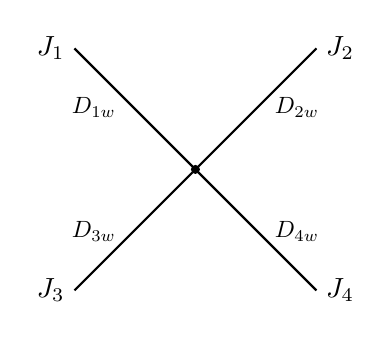
\begin{tikzpicture}[node distance=1.5cm and 1.5cm]
      \coordinate[label=left:$J_1$] (J1);
      \coordinate[vertex,below right=of J1] (w);
      \coordinate[above right=of w,label=right:$J_2$] (J2);
      \coordinate[below left=of w,label=left:$J_3$] (J3);
      \coordinate[below right=of w,label=right:$J_4$] (J4);
      \begin{scope}[every node/.style={scale=.85}]
        \draw[particle] (J1) -- node[label=left:$D_{1w}$] {} (w);
        \draw[particle] (J2) -- node[label=right:$D_{2w}$] {} (w);
        \draw[particle] (J3) -- node[label=left:$D_{3w}$] {} (w);
        \draw[particle] (J4) -- node[label=right:$D_{4w}$] {} (w);  
      \end{scope}
  \end{tikzpicture}
  \end{minipage}
  \begin{minipage}{0.3\textwidth}
    \centering
    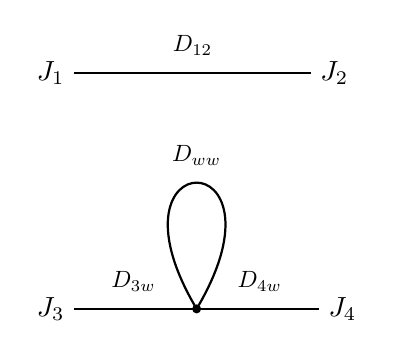
\begin{tikzpicture}[node distance=1.5cm and 1.5cm]
      \coordinate[label=left:$J_1$] (J1);
      \coordinate[right=3cm of J1,label=right:$J_2$] (J2);
      \coordinate[below=3cm of J1,label=left:$J_3$] (J3);
      \coordinate[vertex,right=of J3] (w);
      \coordinate[right=of w,label=right:$J_4$] (J4);
      \begin{scope}[every node/.style={scale=.85}]
        \draw[particle] (J1) -- node[label=above:$D_{12}$] {} (J2);
        \draw[particle] (J3) -- node[label=above:$D_{3w}$] {} (w);
        \draw[particle] (J4) -- node[label=above:$D_{4w}$] {} (w);
        \draw[particle] (w) edge[loop above] node[label=above:$D_{ww}$] {} (w);
      \end{scope}
    \end{tikzpicture}
  \end{minipage}
  \begin{minipage}{0.3\textwidth}
    \centering
    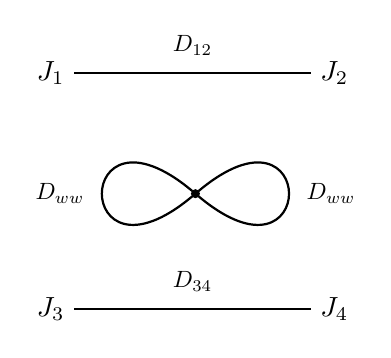
\begin{tikzpicture}[node distance=1.5cm and 1.5cm]
      \coordinate[label=left:$J_1$] (J1);
      \coordinate[right=3cm of J1,label=right:$J_2$] (J2);
      \coordinate[below=3cm of J1,label=left:$J_3$] (J3);
      \coordinate[right=3cm of J3,label=right:$J_4$] (J4);
      \coordinate[vertex,below right=of J1] (w);
      \begin{scope}[every node/.style={scale=.85}]
        \draw[particle] (J1) -- node[label=above:$D_{12}$] {} (J2);
        \draw[particle] (J3) -- node[label=above:$D_{34}$] {} (J4);
        \draw[particle] (w) edge[loop left] node[label=left:$D_{ww}$] {} (w);
        \draw[particle] (w) edge[loop right] node[label=right:$D_{ww}$] {} (w);
      \end{scope}
    \end{tikzpicture}
  \end{minipage}
\end{center}
These diagrams both represent what is physically happening, in
position space, and the terms in the integral. They are also known as
{\bf Feynman diagrams}!

When one does more of these types of calculations for other
$\lambda^k J^n$ terms, one can see many patterns. In each of the three
Feynman diagrams above, there are:
\begin{itemize}
\item one {\bf internal vertex} (the black dot), corresponding to the
  comes from the variable $w$ introduced by the $\lambda^1$ term (if
  we were to compute a $\lambda^k$ term, there would be $k$ internal
  vertices);
\item four {\bf external vertices} coming from the four $J$'s (if we
  were to compute a $J^n$ term, there would be $n$ external vertices);
\item four {\bf propagators} coming from the four $D_F$'s (if we were
  to compute a $J^n$ term, there would be $n$ external vertices).
\end{itemize}

\begin{exercise}
  There are also rules for what possible diagrams can arise in the
  $\phi^4$ theory. Convince yourself that any diagram has:
  \begin{itemize}
  \item four propagator ends at each internal vertex;
  \item an even number of external vertices;
  \item ((number of internal propagators) - (number of internal
    vertices) + 1) loops.
  \end{itemize}
\end{exercise}

So we see that Feynman diagrams are good, intuitive,
easy-to-manipulate representations of the terms of $Z[J, \lambda]$. In
fact, instead of going from a term in $Z[J, \lambda]$ to a Feynman
diagram, we can go the other way: given a Feynman diagram that can
arise from the $\phi^4$ theory, we can directly write down the term
associated to it. This greatly simplifies the calculation of the
terms, since now we can just draw pictures instead of taking $4k$
derivatives $\delta/\delta J(w)$ acting on $2n$ terms $J(x)$.

\begin{theorem}
  Given a Feynman diagram, one can write down its corresponding value
  using the {\bf position-space Feynman rules for $\phi^4$ theory}:
  \begin{itemize}
  \item for each propagator between vertices $x$ and $y$, add a $D_F(x - y)$ term;
  \item for each internal vertex, add a $(-i\lambda) \int d^4z$ term;
  \item for each external vertex, add a factor of $1$;
  \item divide by the {\bf symmetry factor}.
  \end{itemize}
  The symmetry factor is the number of ways of interchanging internal
  components of the diagram without changing the diagram itself.
\end{theorem}

\begin{exercise}
  Symmetry factors take some getting used to. They arise from the
  combinatorics of how the derivatives $\delta/\delta J$ can hit
  different $J$, and the symmetry $D_F(x - y) = D_F(y - x)$. For
  example, when a diagram has a loop in it, we naively overcount by a
  factor of two because of the symmetry in $D_F$. Compute the symmetry
  factors of the following three diagrams using similar reasoning:
  \begin{center}
  \begin{minipage}{0.3\textwidth}
    \centering
    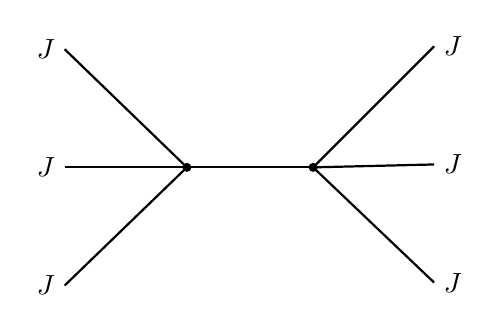
\begin{tikzpicture}[node distance=1.5cm and 1.5cm]
      \coordinate[label=left:$J$] (J1);
      \coordinate[below=of J1,label=left:$J$] (J2);
      \coordinate[below=of J2,label=left:$J$] (J3);
      \coordinate[vertex,right=of J2] (w1);
      \coordinate[vertex,right=of w1] (w2);
      \coordinate[above right=of w2,label=right:$J$] (J4);
      \coordinate[below=of J4,label=right:$J$] (J5);
      \coordinate[below=of J5,label=right:$J$] (J6);
      \begin{scope}[every node/.style={scale=.85}]
        \draw[particle] (J1) -- (w1);
        \draw[particle] (J2) -- (w1);
        \draw[particle] (J3) -- (w1);
        \draw[particle] (w1) -- (w2);
        \draw[particle] (w2) -- (J4);
        \draw[particle] (w2) -- (J5);
        \draw[particle] (w2) -- (J6);
      \end{scope}
    \end{tikzpicture}
  \end{minipage}
  \begin{minipage}{0.3\textwidth}
    \centering
    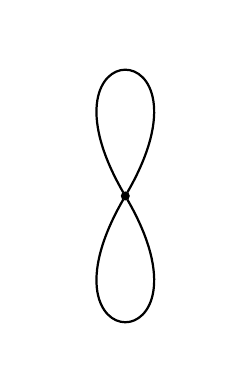
\begin{tikzpicture}[node distance=1.5cm and 1.5cm]
      \coordinate[vertex] (w);
      \begin{scope}[every node/.style={scale=.85}]
        \draw[particle] (w) edge[loop above] (w);
        \draw[particle] (w) edge[loop below] (w);
      \end{scope}
    \end{tikzpicture}
  \end{minipage}
  \begin{minipage}{0.3\textwidth}
    \centering
    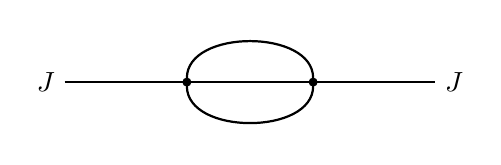
\begin{tikzpicture}[node distance=1.5cm and 1.5cm]
      \coordinate[label=left:$J$] (J1);
      \coordinate[vertex,right=of J1] (w1);
      \coordinate[vertex,right=of w1] (w2);
      \coordinate[right=of w2,label=right:$J$] (J2);
      \begin{scope}[every node/.style={scale=.85}]
        \draw[particle] (J1) -- (w1);
        \draw[particle] (w1) edge[in=90,out=90] (w2);
        \draw[particle] (w1) -- (w2);
        \draw[particle] (w1) edge[in=-90,out=-90] (w2);
        \draw[particle] (w2) -- (J2);
      \end{scope}
    \end{tikzpicture}
  \end{minipage}
  \end{center}
  You should get $1$ and $2 \cdot 2 \cdot 2 = 8$ and $3! = 6$
  respectively.
\end{exercise}

\begin{exercise}
  Rewrite the position-space Feynman rules in momentum-space, to
  obtain the {\bf momentum-space Feynman rules for $\phi^4$ theory}:
  \begin{itemize}
  \item for each internal propagator, label it with a momentum $p$ and
    add a $i/(p^2 - m^2 + i\epsilon)$ term;
  \item for each external propagator (i.e. source), label it with a
    momentum $p$ and add a $e^{-ipx}$ term;
  \item for each internal vertex, add a $-i\lambda$ term;
  \item for each vertex, impose momentum conservation by adding a
    $\delta^{(4)}(p_1 + p_2 - p_3 - p_4)$ term, where
    $p_1, p_2, p_3, p_4$ are the four propagators entering/leaving the
    vertex;
  \item integrate over every undetermined momentum $p$ with
    $\int d^4p/(2\pi)^4$;
  \item divide by the symmetry factor.
  \end{itemize}
  Note that in momentum space, we must orient each propagator. The
  orientation is arbitrary, since $D_F(x - y) = D_F(y - x)$, but
  necessary for imposing momentum conservation.
\end{exercise}

\section{Connected vs Disconnected}



\chapter{Quantum Electrodynamics}
\section{Functional Quantization of Spinor Fields}
Now that we have understood the essentials of the path integral formulation
we would now like to apply this formalism to understand how fermions
interact in an electromagnetic field. Before we can get anywhere let us
revisit the Dirac field and attempt to quantize it using the path integral
formalism. 

Recall that in our discussion of the Dirac field we realized that fermionic
quantization required anticommutation relations. This suggests that the
eigenfunctions of these operators also need to anticommute. These sorts of
variables are called Grassmann numbers: $\theta\eta = -\eta\theta$. To
proceed, we first need to understand how to integrate over such variables.
It will turn out that integration over these variables is much easier than
regular integration! Consider the Taylor expansion $f(\theta) = A +
B\theta+C\theta^2+D\theta^3 + \cdots$. If $\theta$ is a Grassmann variable
then $\theta^2=0$ and so $f(\theta) = A + B\theta$. The two properties that
we would like of integration is that it is linear and invariant under a
translation of variables, $\theta\to \theta+\eta_0$. Thus:
\begin{align*}
    \int d\theta\, f(\theta) &= \int d\theta\,A+B\theta
    = \int d(\theta+\eta_0)\, A+B(\theta+\eta_0)\\
    &= \int d\theta\, (A+B\eta_0) + B\theta
\end{align*}
By linearity, we expect that this integral be a linear function of the
constant term, $A$, and the linear term, $B$. The last equality implies that 
The integral does not depend on the constant term. Therefore, we may assume
that the integral evaluates to:\footnote{Integration by differentiation!}
\begin{align*}
    \int d\theta\, A+B\theta = B
\end{align*}
If we integrate more than one Grassmann number we need the following
convention that $\int d\eta\int d\theta\,\theta\eta = 1$.
This definition makes some integrals very easy to evaluate. We compile a
few that will be useful for us later on:
\begin{align}
    \int d\theta^* d\theta e^{-\theta^* b\theta} &= b^{-1}, &
    \left(\prod_i\int d\theta_i^*d\theta_i\right)
    e^{-\theta_i^*B_{ij}\theta_j} = \prod_i b_i &= \det B, &
    \left(\prod_i\int d\theta_i^*d\theta_i\right)
{\color{red}\theta_k\theta_l^*e^{-\theta_i^*B_{ij}\theta_j}} &= (\det
B)(B^{-1})_{kl}
    \label{fermionic-integrals}
\end{align}

Recall that the Lagrangian for the Dirac field is given by $\mc L_{Dirac} =
\bar\psi (i\slashed\di - m) \psi$ where $\slashed\di = \gam^\mu\di_\mu$.
Using the integrals given in \eqref{fermionic-integrals} it is possible to
immediately calculate the correlation functions for the free field theory
directly. Instead, we will get some more practice with our generating
functional method.

\begin{comment}
%   {\color{blue} (Blue colour means skip during the lecture, and possibly skip
%   in these notes.
%
%   Using the integrals given in \eqref{fermionic-integrals} we may calculate
%   the two-point correlation function immediately:
%   \begin{align*}
%       \braket{0|T\psi(x_1)\bar\psi(x_2)|0}
%   &=\FR{\int D\bar\psi D\psi\,\psi(x_1)\bar\psi(x_2)e^{i\int d^4x\bar\psi(i\slashed\di-m)\psi}}
%        {\int D\bar\psi D\psi\,e^{i\int d^4x\bar\psi(i\slashed\di-m)\psi}}\\
%        &=\FR{\det (i\slashed\di-m)\cdot
%            \braket{\bar\psi(x_2)|\bigl\{-i(i\slashed\di-m)\bigr\}^{-1}|\psi(x_1)}}
%            {\det (i\slashed\di-m)}
%   \end{align*}
%   The inverse operator is the Green's function for the Dirac equation, which
%   can be computed by Fourier transforming.
%   \begin{align*}
%   \delta^{(4)}(x-y) &= -i(i\sdi-m)\cdot G(x-y)\\
%   &= -i(i\sdi-m)\int\FR{d^4p}{(2\pi)^4} e^{-ip(x-y)}\tilde G(p)\\
%   &= \int \FR{d^4p}{(2\pi)^4} (-i\slashed{p}+im)\tilde G(p)e^{-ip(x-y)}\\
%   1 &= (-i\slashed{p}+im)\tilde G(p)\implies G(x-y) = \int\FR{d^4p}{(2\pi)^4}
%   \FR{ie^{-ip(x-y)}}{\slashed p - m+i\epsilon}
%   \end{align*}
%   Therefore,
%   \begin{align*}
%   \braket{0|T\psi(x_1)\bar\psi(x_2)|0} &= \int\FR{d^4p}{(2\pi)^4} 
%   \FR{ie^{-ip(x_1-x_2)}}{\slashed{p}-m+i\epsilon}= S_F(x_1-x_2)
%   \end{align*}
%   where the pesky $i\epsilon$ came in because of {\color{red}convergence
%   issues}.}
\end{comment}
Take the generating functional,
\begin{align*}
Z[\bar\eta,\eta] = \int D\bar\psi D\psi 
\exp\left[ i\int d^4x\,\bar\psi(i\sdi-m)\psi + \bar\eta\psi+\bar\psi\eta
\right]
\end{align*}
So that if you make the substitution $\psi \to \psi+(i\sdi-m)^{-1}\bar\eta$
then we can evaluate $Z$ explicitly:
\begin{align*}
Z[\bar\eta,\eta] =  Z_0\cdot \exp\left[ -\int d^4xd^4y
\bar\eta(x)S_F(x-y)\eta(y) \right]
\end{align*}
Therefore we are in position to evaluate arbitrary $n$-point correlation
functions. This is where the generating functional method shines, on the
one hand it is easy to compute explicitly, and on the other hand by
differentiating it in a special way it gives rise to the correlation
functions! In the free field case, here is an example of such a correlation
function calculation:
\begin{align*}
    \braket{0|T\psi(x_1)\psi(x_2)|0} = 
    Z_0^{-1} \cdot \left(
    \FR{-i\delta}{\delta\bar\eta(x_1)}
    \right)\left( \FR{+i\delta}{\delta\eta(x_2)}\right) Z[\bar\eta,\eta] 
        =
    \left(
    \FR{-i\delta}{\delta\bar\eta(x_1)}
    \right)\left( \FR{+i\delta}{\delta\eta(x_2)} \right)
\exp\left[ -\int d^4xd^4y
\bar\eta(x)S_F(x-y)\eta(y) \right]
\end{align*}
What are possible interactions that we can add to the Dirac field? Since
we've already discussed the scalar field, we may start by coupling the
Dirac field to the scalar field and trying to compute the correlation
functions.

% Yukawa and Coulomb potential will be discussed at the end.

To talk about QED we need the quantized version of the electromagnetic
field. Here we go!
\section{Functional Quantization of Electromagnetic Field}
\colr{sketch}

The electromagnetic field is described by a 4-vector, $A_\mu = (\phi,\vec
A)$, which packages the information about the electric field into $\phi$
and the magnetic field into $\vec A$. By taking the Lagrangian: $\mc L_{EM}
=-\FR{1}{4}F_{\mu\nu}F^{\mu\nu}$, where $F_{\mu\nu} = \di_\mu A_\nu
-\di_\nu A_\mu$, we recover Maxwell's equations (exercise!). We may write
the action explicitly in terms of the $A_\mu$:
\begin{align*}
    \int d^4x \mc L_{EM} &= \int d^4x\, -\FR{1}{4}F_{\mu\nu}F^{\mu\nu}\\
    &= -\FR{1}{4} \int d^4x\, \left( \di_\mu A_\nu - \di_\nu A_\mu \right)
    \left( \di^\mu A^\nu - \di^\nu A^\mu \right)\\
    &= \FR{1}{2}\int d^4x\, A_\mu(\di^2g^{\mu\nu} -\di^\mu\di^\nu) A_\nu
\end{align*}
Fourier transforming the variables, $A_\mu$, would get:
\[ 
    \int d^4x \mc L_{EM} =
    \FR{1}{2}\int \FR{d^4k}{(2\pi)^4}\, A_\mu(k^2g^{\mu\nu} -k^\mu k^\nu) A_\nu
\]
The $4\times 4$ matrix $(k^2g^{\mu\nu} -k^\mu k^\nu)$ is not invertible and
so


Change of variables
\[ \int_{\bR^n} dx\, \delta(g(x))|g'(x)|f(g(x)) = \int_{g(\bR^n)} du
\delta(u)f(u) \]
which means that we can interpret $\int_{\bR^n} dx\, \delta(g(x))|g'(x)|$
as taking a constant function and returning the constant function back. So 
\begin{align*}
1 &= \int_{\bR^n} dx\, \delta(g(x))|g'(x)|\\
1 &= \int \mc D\alpha(X) \delta(G(A^\alpha))
\det\PFR{\delta G(A^\alpha)}{\delta\alpha}
\end{align*}
Note $\det\PFR{\delta G(A^\alpha)}{\delta\alpha} = \det(\partial^2/e)$
Then \begin{align*}
    \int \mc DA e^{iS[A]}
&= \det\PFR{\delta G(A^\alpha)}{\delta\alpha}
\int \mc D\alpha\int \mc D A e^{iS[A]}\delta(G(A^\alpha))\\
&= 
\det(\partial^2/e) \left( \int\mc D\alpha \right)
\int \mc D A^\alpha e^{iS[A^\alpha]}\delta(G(A^\alpha))
\end{align*}
Take a general gauge-fixing condition, $G(A) = \di^\mu A_\mu(x) -
\omega(x)$ for scalar function $\omega$. The above holds for any linear
combination of $\omega$'s so that we may take a very big linear
combination, weigted by a Gaussian:
\begin{align*}
    \int \mc DA e^{iS[A]}
    &= \underbrace{N(\xi) \int D\omega \exp \left[ -i\int d^4x
    \FR{\omega^2}{2\xi} \right]}_{=1}
\det(\partial^2/e) \left( \int\mc D\alpha \right)
\int \mc D A e^{iS[A]}\delta(\di^\mu A_\mu - \omega(x))\\
&= N(\xi) \det(\partial^2/e) \left( \int\mc D\alpha \right)
\int \mc D A e^{iS[A]} \exp \left[ -i\int d^4x \FR{(\di_\mu A^\mu)^2}{2\xi}\right]\\
&= N(\xi) \det(\partial^2/e) \left( \int\mc D\alpha \right)
\int \mc D A \exp \left[ \FR{i}{2}\int d^4x\, A_\mu(\di^2g^{\mu\nu}- \di^\mu\di^\nu)A_\nu\colr{-\FR{(\di_\mu A^\mu)^2}{\xi}}\right]\\
&= N(\xi) \det(\partial^2/e) \left( \int\mc D\alpha \right)
\int \mc D A \exp \left[ \FR{i}{2}\int d^4x\, A_\mu(\di^2g^{\mu\nu}-\di^\mu\di^\nu)A_\nu\colr{+\FR{A_\mu\di^\mu\di^\nu A_\nu}{\xi}}\right]\\
&= N(\xi) \det(\partial^2/e) \left( \int\mc D\alpha \right)
\int \mc D A \exp \left[ \FR{i}{2}\int d^4x\, A_\mu(\di^2g^{\mu\nu}
-\left(1-\FR{1}{\xi}\right)\di^\mu\di^\nu)A_\nu\right]\\
&\propto
\int \mc D A \exp \left[ \FR{i}{2}\int \FR{d^4k}{(2\pi)^4}\,
A_\mu(k^2g^{\mu\nu}-\left(1-\FR{1}{\xi}\right)k^\mu k^\nu)A_\nu\right]\\
\end{align*}

Inverting,
\[D^\gam_F(k)=\FR{-i}{k^2+i\epsilon}(g^{\mu\nu}-(1-\xi)\FR{k^\mu k^\nu}{k^2}\]
The full free field QED Lagragian will then be of the form:
\[ Z[J_\mu,\bar\eta,\eta] = \exp\left[ \FR{-1}{2}\int d^4x d^4y\, \bar\eta
S_F(x-y) \eta + J_\mu (D^\gam_F)^{\mu\nu} J_\nu \right] \]
\subsection{Interaction term: Fermions and Photons}
Let's guess the interaction term:
\begin{itemize}
    \item $\psi$ is a column vector, $\bar\psi$ is a row vector.
    \item $A_\mu$ is a column vector.
    \item $\gam^\nu$ are four matrices
\end{itemize}
After a bit of fiddling there are a few simple choices, up to prefactors,
\[\bar\psi\psi\slashed A, \bar\psi\psi A^2, \bar\psi\gam^\mu\psi A_\mu.\]
But there are many higher order terms. How do we exclude these terms
theoretically? I mean, we don't have to: we can guess one model, realize
that it agrees well with experiment and be done. However, it's possible to
theoretically justify why the simplest theory ought to be the correct one.
This is the argument of \textbf{renormalizability}.

\subsubsection{Introduction to Renormalizable Theories}
Higher order terms in perturbation theory can be computed using integrals
over $4$-momenta. These integrals are seemingly divergent, so we 
\begin{enumerate}
    \item Introduce a large cutoff $\Lambda$.
    \item Evaluate integral.
    \item Take $\Lambda\to\infty$, hope answer is independent of $\Lambda$.
\end{enumerate}
A theory in which this procedure works are called renormalizable. Whether a
theory is or is not renormalizable can be heuristically checked by a
dimensional analysis.

Using $E = 2\pi\hbar \nu = pc = p = mv = m$ and $L/T = c = 1$ we list two
relations that are useful for us:
\begin{align*}
    L &= T\\
    T^{-1} &= [p] = M
\end{align*}
The momentum cutoff has units, $[\Lambda]=[p]=M$. Moreover the Lagrangian
has units of $M^4$ since
\begin{itemize}
    \item Action dimensionless, $S = e^{i\int d^4x \mc L}$
    \item so $1 = [Length]^4\cdot [\mc L] = [M]^{-4}[\mc L]$.
\end{itemize}
Examples of dimensions. 
\begin{itemize}
    \item 
$\mc L = \FR{1}{2}\di^2\phi - \FR{1}{2}m^2\phi^2 \implies [\phi] = M$.
    \item 
$\mc L = \bar\psi(i\slashed\partial-m)\psi \implies [\bar\psi m \psi] =
M^4, [\psi] = M^{3/2}$.
    \item
$\mc L = F^2 = A_\nu\di^2g^{\mu\nu}A_\mu + \dots \implies
[A^2\di^2] = [A^2m^2] = M^4 \implies [A_\mu]=M$
\end{itemize}
Scattering amplitudes.
\[\colr{[\textrm{Coupling const.}] \sim \FR{1}{M^k}\implies [Sc. Ampl] \sim \FR{1}{M^k}\cdot
\Lambda^k\to\infty.}\]

To combine $\psi$ and $A_\mu$ we need: 

\[\colr{[\textrm{Coupling const.}]}\cdot [\psi]^k [A_\mu]^\ell =
M^cM^{3k/2} M^\ell=1\]
so
\[ 3k/2+\ell \le 4 \iff (k,\ell)\in\{ (1,1), (2,1) \}.\]


\section{Aside: Scattering Amplitudes}
Let us briefly try to understand the big picture -- or, in fact, I guess it's the
small picture! A \textbf{cross section} is the fundamental physical
quantity that an experimental particle physicist is interested in, here's
roughly what it is. Suppose you want to understand the inner workings of
protons. You will devise an experiment to smash some number of protons
together and try to investigate the result. In fact, your theorist friends
suggest to you some possible types of particles that can come out.
Ideally, if we're not in one already, we will consider two protons
colliding to produce other species: $pp \to abc\ldots$.

Your detectors cover only a portion of $4\pi$, as the experimentalists call
it, that is, the sphere surrounding the collision point. Therefore, we
would like to compute the amount of scattering events in the direction of
the detector. This is given the symbol:
\[ \PFR{d\sigma}{d\Omega} \]
This is a very technical object and it depends on a lot of parameters.
Qualitatively, we may simplify this object by considering just the
\textbf{scattering events} which are partly characterized by momenta
(particle type, spin, etc. are also valid quantum numbers). The scattering
events can be analyzed by looking at the \textbf{S-matrix}:
\begin{align*}
\braket{\vec p_1\cdots|S|k_Ak_B}&:=
{}_{\text{out}}\braket{\vec p_1\vec p_2\cdots|\vec k_A\vec k_B}_{\text{in}}\\
&= \lim_{T\to\infty} \braket{\vec p_1\cdots|e^{iH(2T)}|\vec k_A\vec k_B}
\end{align*}
In words, this means that we assume that our particles are idealized
momentum eigenstates and long after they interact they again will be
idealized momentum eigenstates. We apply a trick, that sometimes particles
don't interact at all, and we can take that out of the $S$ matrix:
\[ S = \iden + i T \]
Assuming unitarity of $S$ (which is a big assumption!) $T$ is a Hermitian
operator (think of $e^{i\theta}$) and it contains all of the interesting
dynamics. By also considering energy conservation can be written as:
\[
\braket{p_1\dots| iT |k_Ak_B} 
=(2\pi)^4\delta^{(4)}(k_A+k_B-\sum p_f) \mc M(k_A,k_B\to\{p_f\})
\]
What this means is that the scattering amplitude is really a distribution
and the density is given by the expression $\mc M$. To briefly connect this
back to the cross section, in the case that there are four identical
particles (two incoming and two outgoing) then the cross section will be
(PS 4.85)
\[ \PFR{d\sigma}{d\Omega}_{CM} = \FR{|\mc M|^2}{64\pi^2E_{cm}^2}.\]
\subsection{Scattering amplitudes via Feynman diagrams}
Now we interpret the scattering amplitude as something very similar to a
correlation function. Recall a correlation function for us was
\begin{align}
\braket{\Omega|T\{\phi(x_1)\phi(x_2)\}|\Omega}
&= \lim_{T\to\infty(1-i\epsilon)}
\FR{ \int D\phi\, \phi(x_1)\phi(x_2) \exp[i\int_{-T}^T \mc L] }
{ \int D\phi\, \exp[i\int_{-T}^T \mc L] } \label{fcnintcorfcn}\\
&= 
\lim_{T\to\infty(1-i\epsilon)}
\FR{\braket{0|T\{\phi(x_1)\phi(x_2)\exp[-i\int_{-T}^Tdt\,H_I(t)]\}|0}}
{\braket{0|T\{\exp[-i\int_{-T}^Tdt\,H_I(t)]\}|0}}
\label{canqntcorfcn}
\end{align}
Although we haven't explicitly mentioned this in our lectures, the formula
in line \eqref{canqntcorfcn} has appeared in the derivation of
\eqref{fcnintcorfcn} (see \eqref{tricky} to compare). 

Here's a quick review of how we derived a path integral representation for
the correlation functions:
\begin{itemize}
    \item Using a leap of intuition we define (or is it prove?)
        \[ \braket{\phi(a)|e^{-iHt}|\phi(b)} = \int \mc D\phi
            \exp \left[ i\int d^4x \mc L \right] \]
    \item Investigate the expression
        \[ \int \mc D\phi\, \phi(x_1)\phi(x_2) \exp \left[ i\int d^4x \mc
        L\right] \]
        by splitting up the path into three sections.
    \item Simplify this to get 
\begin{align} \bra{\phi_b(\vec{x})} e^{-i\hat{H}(t - x_2^0)} \phi(\vec{x}_2)
    e^{-i\hat{H}(x_2^0 - x_1^0)} \phi(\vec{x}_1) e^{-i\hat{H}(x_1^0 -
(-t))} \ket{\phi_a(\vec{x})}
\end{align}
    \item The Canonical Quantizers prefer to rewrite this expression up to
        prefactors (which come from approximating $\phi_{a,b}(\vec x)$ with
        $\ket\Omega$):
\[
\braket{0|T\left\{\phi_I(x_1)\phi_I(x_2)\exp[-i\int_{-T}^Tdt\,H_I(t)]\right\}|0}
\]
        The extra $I$'s on the $\phi$'s absorb the free evolution into the
        original $\phi$'s. 
\end{itemize}

Now we may interpret the scattering amplitude as the following:
\begin{align}\braket{\vec p_1\ldots\vec p_n|iT|\vec p_A\vec p_B}
&=\lim_{T\to\infty(1-i\epsilon)} {}_0\braket{\vec p_1\ldots\vec p_n
|e^{-iH(2T)}|\vec p_A\vec p_B} { }_0\\
&\propto\lim_{T\to\infty(1-i\epsilon)} \left( {}_0\braket{\vec p_1\ldots\vec p_n
|T\exp\left[ -i\int_{-T}^T dt\, H_I(t) \right]|
\vec p_A\vec p_B} { }_0 \right)_\text{connected, amputated}
\label{Smatrix}
\end{align}
The zeros on the end of the bracket refer to idealistic wavepackets. 


\subsection{Wick's Theorem}
Our next goal will be to interpret this amplitude as a sum of Feynman diagrams.
We will now introduce \textbf{Wick's theorem}, and thus \textbf{Wick
contractions}, using which we'll be able to write down the Feynman diagrams
very easily.

In canonical quantization there are raising and lowering operators. 
We introduce a particular order for expressions involving operators:
raising on the left and lowering on the right -- \textbf{Normal Order}.
A Wick contraction is defined by:
\[ \begC1{\phi(x)}\conC{}\endC1{\phi(y)} = D_F(x-y) \]
Finally Wick's theorem states the following:
\begin{theorem}
    \[T\{ \phi(x_1)\phi(x_2)\cdots\phi(x_n) \}
    =N\{ \phi(x_1)\phi(x_2)\cdots\phi(x_n) + \text{all possible
    contractions}\}\]
\end{theorem}
This is a theorem with very major \emph{computational} consequences for
physics. In particular, this makes the Feynman diagrams immediate!
Let's go through an example from Peskin and Schroeder:
\begin{align*}
    &{\ }\braket{0|T\left\{ \phi(x)\phi(y) + \phi(x)\phi(y)
        \left[ -i\int dt \int d^3z \FR{\lam}{4!} \phi(z)^4 \right]
        +\cdots
    \right\}|0}\\
    &= \braket{0|T\{\phi(x)\phi(y)\}|0}
    +\FR{(-i\lam}{4!}\braket{0|T\{\phi(x)\phi(y)\phi(z)\phi(z)\phi(z)\phi(z)|0}\\
\end{align*}
Apply Wick's Theorem:
\begin{align*}
    &{\ } \braket{0|N\{\phi(x)\phi(y) +
        \colf{\begC1{\phi(x)}\endC1{\phi}(y)}\}|0}\\
        &+\FR{(-i\lam)}{4!}\braket{0|N\{\phi(x)\phi(y)\phi(z)\phi(z)\phi(z)\phi(z)\}|0}\\
        &+\FR{(-i\lam)}{4!}\braket{0|N\{\begC1{\phi(x)}\endC1{\phi(y)}\phi(z)\phi(z)\phi(z)\phi(z)\}|0}\\
        &+\FR{(-i\lam)}{4!}\braket{0|N\{\begC1{\phi(x)}\conC{\phi(y)}\endC1{\phi(z)}\phi(z)\phi(z)\phi(z)\}|0}+\cdots \\
        &+\FR{(-i\lam)}{4!}\braket{0|N\{\begC1{\phi(x)}\endC1{\phi(y)}\begC1{\phi(z)}\endC1{\phi(z)}\phi(z)\phi(z)\}|0}+\cdots\\
        &+\colf{\FR{(-i\lam)}{4!}\braket{0|N\{\begC1{\phi(x)}\begC2{\phi(y)}\endC1{\phi(z)}\endC2{\phi(z)}\begC1{\phi(z)}\endC1{\phi(z)}\}|0}}+\cdots\\
\end{align*}
Now you can probably see where the Feynman Diagrams will be appearing! They
In fact, using this approach I would hazard that it's even easier to see
where the Feynman diagrams are coming from! Because of the normal ordering
most of these are zero, in fact only the Fuchsia coloured terms are
non-zero.

Let's apply these rules to calculate the scattering amplitude (finally!).
One last rule before we do this, since $\ket{\vec p} \propto a^\dag_{\vec
p}\ket0$, it makes sense to define:
\[
    \begC1{\phi(x)}\endC1{\ket{p}} = e^{-ip\cdot x}
    \qquad\qquad
    \begC1{\bra{p}}\endC1{\phi(x)} = e^{+ip\cdot x}
\]
Now, we compute a few examples. NOTE: the first amplitude does \textbf{not}
have a time ordering so we compute it directly.
\begin{align*}
    \braket{p_1p_2|p_Ap_B} &= \sqrt{2E_12E_2 2E_A
    2E_B}\braket{0|a_1a_2a_A^\dag a_B^\dag|0} = (diagram) \\
    \braket{p_1p_2|\mc T \left\{  \FR{(-i\lam)}{4!}\int d^4x
\phi_x\phi_x\phi_x\phi_x\right\}|p_Ap_B} 
&=  \FR{(-i\lam)}{4!}\int d^4x\biggl(
\colb{(\ )\times \braket{p_1p_2|\begC1{\phi_x}\endC1{\phi_x}\begC1{\phi_x}\endC1{\phi_x}|p_Ap_B}}\\ 
&\colb{+(\ )\times \braket{p_1\begC1{p_2|}\endC1{\phi_x}\begC1{\phi_x}\endC1{\phi_x}\begC1{\phi_x|}\endC1{p_A}p_B}}\\
&\colf{+(4!)\times\braket{\begC2{p_1}\begC1{p_2|}\endC1{\phi_x}\endC2{\phi_x}\begC2{\phi_x}\begC1{\phi_x|}\endC1{p_A}\endC2{p_B}}}\\
\end{align*}
The blue terms are not interesting. The very first term is just zero
because they contribute to the $\iden$ in $S = \iden + iT$; the second blue
term is also not interesting because it also contributes to the $\iden$.
The fuchsia term is very interesting because by applying the rules that
we've expressed above we get:
\[\braket{p_1p_2|iT|p_Ap_B} 
\approx\FR{-i\lam}{4!}\int d^4x\, (4!)\times e^{i(p_1+p_2-p_A-p_B)\cdot x}
= \colb{(-i\lam)}\cdot (2\pi)^4\delta^{(4)}(p_1+p_2-p_A-p_B) \]
But we also had,
\[\braket{p_1p_2|iT|p_Ap_B} 
= \colb{i\mc M(p_1p_2\to p_Ap_B)} \cdot (2\pi)^4\delta^{(4)}(p_1+p_2-p_A-p_B) \]

%   And here's a complicated example using all three levels:
%   $$
%   \langle0|\, \begC2{\phi(x)}\begC3{\phi(y)}\conC{\,{1\over3!}
%     \bigl({-i\lambda\over4!}\bigr)^3\int\!d^4z\,}\endC2{\phi}\begC1{\phi}
%     \endC1\phi\begC1\phi\conC{\,\int\!d^4w\,}\endC1\phi\begC2\phi
%     \begC1\phi\endC3\phi\conC{\,\int\!d^4u\,}\endC1\phi\endC2\phi
%     \begC1\phi\endC1\phi\,|0\rangle
%   $$


\section{Amplitudes from QED}
How do we handle any other theory? We have developed two procedures: first
we wrote down the scattering amplitude; second we drew a Feynman diagram
associated to it. Ideally, we'd like to go the other way because drawing
diagrams is easier. But in order to do this we need to know the (Feynman)
rules, of what we need to replace each arrow or vertex in the propogator
by. 

In the spin-0 theory, I defined the Wick contraction to be $D_F(x-y)$,
but for other particles, we replace this with the associated propogator.
The vertex terms can be read off the interaction Hamiltonian. All of the
subtle points, always go back to the expression for the scattering
amplitude and computed directly; the passage to the combinatorial Feynman
diagrams is for now just a convenient representation. Without further ado,
let's begin QED. 

Let's quickly recall that all solutions to the Dirac equation can be spin
up or down and the general Dirac field can be written as in \eqref{ferm1}
and \eqref{ferm2}, which we remind ourselves here:
\begin{align*} 
\psi(x) &= \int \FR{d^3p}{(2\pi)^3} 
\ha^{s}_\vp u^s(\vp) e^{-i\vp\cdot\vx} +
\hb^{s\dag}_\vp v^s(\vp) e^{i\vp\cdot\vx}, &
\bar\psi(x) &= \int \FR{d^3p}{(2\pi)^3} 
\hb^{s}_\vp \bar v^s(\vp) e^{-i\vp\cdot\vx} +
\ha^{s\dag}_\vp \bar u^s(\vp) e^{i\vp\cdot\vx}, & \text{where}\ s&=1,2
\end{align*}

\subsubsection{Feynman Rules for QED}
\begin{enumerate}
        \color{blue}
    \item Propogators:
        \begin{align*}
            \begC1{\psi}\conC{(x)}\endC1{\bar\psi}(y) &= \FR{i}{\slashed
            p-m+i\epsilon}\\
            \begC1{A_\mu}\conC{(x)}\endC1{A_\nu}(y) &=
            \FR{-ig_\mu\nu}{q^2+i\epsilon}
        \end{align*}
    \item Vertex: $-ie$.
    \item External legs contractions (for more details and Feynman diagrams
        see Peskin and Schroeder pg 118, 123):
\begin{align*}
\begC1{\psi(x)}\endC1{\underbrace{\ket{p,s}}_{\text{fermion}}} &= u^s(p)\ket 0 &
\begC1{\underbrace{\bra{p,s}}_{\text{fermion}}}\endC1{\bar\psi(x)} &= \bar u^s(p)\ket 0\\
\begC1{\bar\psi(x)}\endC1{\underbrace{\ket{k,s}}_{\text{antifermion}}}&=v^s(k)\ket 0 &
\begC1{\underbrace{\bra{k,s}}_{\text{antifermion}}}\endC1{\psi(x)}&=v^s(p)\ket 0\\
\begC1{A_\mu}\endC1{\ket{p}}&= \epsilon_\mu(p) &
\begC1{\bra{p}}\endC1{A_\mu}&= \epsilon_\mu^*(p)
\end{align*}
\item Impose momentum conservation at each vertex.
\item Integrate over each undetermined loop momentum.
%\item Figure out the overall sign of the diagram.
\end{enumerate}
Thus, a typical matrix element is given by
\begin{align*}
    \braket{\begC2{p_1}\begC1{p_2|}\conC{\int{d^3x}}\endC1{\bar\psi}\conC{\gam^\mu}\begC1{\psi}\begC3{A_\mu}\conC{\cdot}\endC2{\bar\psi}\conC{\gam^\nu}
    \begC2{\psi}\endC3{A_\nu}\conC{|}\endC1{p_A}\endC2{p_B}}
    &= (\int\colb{d^4q}) \cdot (-ie)^2
    \bar u(p_2)\gam^\mu u(p_A)
    \PFR{-ig_{\mu\nu}}{q^2+i\epsilon}
    \bar u(p_1)\gam^\nu u(p_B)\\
    &.\qquad\qquad\times
    (2\pi)^8
    \delta^{(4)}(p_A+q-p_1)
    \delta^{(4)}(p_B+q-p_2)\\
    &= i\mc M\times (2\pi)^4\delta^{(4)}(p_A+p_B-p_1-p_2)
\end{align*}
where the diagram corresponding to this choice of contractions is given by:
%   \begin{center}
%   \begin{fmffile}{diagram}
%       \begin{fmfgraph}(100,160)
%           \fmfleft{i1,i2}
%           \fmfright{o1,o2}
%           \fmf{fermion}{i1,v1,i2}
%           \fmf{fermion}{o1,v2}
%           \fmf{photon}{v1,v2}
%       \end{fmfgraph}
%   \end{fmffile}
%   \end{center}
\vspace{4cm}
\subsubsection{Born Approximation}
In the nonrelativistic regime, one has the following identity:
\[ \braket{\vec p|iT|\vec q} =-i V(\vec p-\vec q)\delta(E_p-E_q) \]
In the case of the $e^-e^- \to e^-e^-$ vertex that we computed above we get 
\[ V(x) = -\FR{e^2}{4\pi r} \]
which is the Coulomb repulsion that we are familiar.

\chapter{Renormalization}

There is a problem with the machinery we have been developing that we
have been sweeping under the rug. This problem is best illustrated by
explicitly computing the following Feynman diagram for $\phi^4$ theory
(it is the only second-order interaction we are interested in when
computing $4$-particle scattering amplitudes):
\begin{center}
  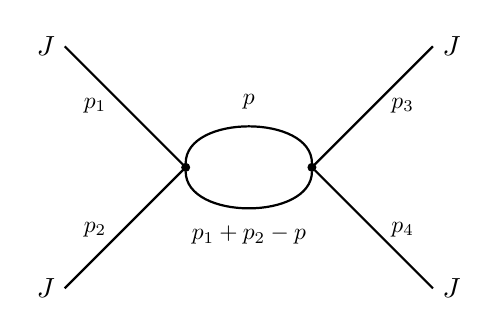
\begin{tikzpicture}[node distance=1.5cm and 1.5cm]
    \coordinate[label=left:$J$] (J1);
    \coordinate[vertex,below right=of J1] (w1);
    \coordinate[below left=of w1,label=left:$J$] (J2);
    \coordinate[vertex,right=of w1] (w2);
    \coordinate[above right=of w2,label=right:$J$] (J3);
    \coordinate[below right=of w2,label=right:$J$] (J4);
    \begin{scope}[every node/.style={scale=.85}]
      \draw[particle] (J1) -- node[label=left:$p_1$] {} (w1);
      \draw[particle] (J2) -- node[label=left:$p_2$] {} (w1);
      \draw[particle] (w1) edge[in=90,out=90] node[label=above:$p$] {} (w2);
      \draw[particle] (w1) edge[in=-90,out=-90] node[label=below:$p_1+p_2-p$] {} (w2);
      \draw[particle] (w2) -- node[label=right:$p_3$] {} (J3);
      \draw[particle] (w2) -- node[label=right:$p_4$] {} (J4);
    \end{scope}
  \end{tikzpicture}
\end{center}
Here we've labeled each source and propagator with its momentum, where
since $p$ is an internal momentum, we must integrate over it. The
value of the diagram is
$$ \frac{(-i\lambda)^2}{2} \int \frac{d^4p}{(2\pi)^4} \frac{i}{p^2 - m^2 + i\epsilon} \frac{i}{(p_1 + p_2 - p)^2 - m^2 + i\epsilon}. $$
As $|p| \to \infty$, the integrand is $O(1/p^4)$, which diverges
logarithmically when integrated over! This divergence cannot simply be
ignored, since it does not get absorbed into the $Z[0,0]$ constant
that we can ignore; it is part of a $J^4$ term. In fact, there are
many such divergences. An easy observation is that any diagram with
this diagram as a sub-diagram will have the same divergence. So we
must develop a way to remove these divergences, or, rather, explain
why they come about in our naive theory, and how to avoid them in a
more sophisticated theory. In this chapter, we will develop such a
theory and systematically remove these divergences using {\bf
  renormalization theory}.

\section{Counting Divergences}

The first step to getting rid of divergences is to understand what
kind of divergences occur, and this we will do by analyzing the
divergent Feynman diagrams. For this section, we will work in $d$
dimensions (instead of $4$) to make the general structure of the
results clearer.

Why did the above diagram diverge? The obvious answer is that there
weren't enough powers of $p$ in the denominator.

\begin{definition}
  The {\bf superficial degree of divergence} $D$ is the difference
  $$ D = \text{(power of } p \text{ in numerator)} - \text{(power of } p \text{ in denominator)}. $$
  Every integration $dp$ counts as a power of $p$ in the numerator. If
  $D \ge 0$, we say the integral is {\bf superficially divergent}.
\end{definition}

If $D \ge 0$ then surely the integral is divergent. However, this is
not an if and only if. For example, take
$\iint dx \, dy \, 1/(1 + x^2)^2$ in $\bR^2$, for which $D = -2$, yet
the integral still diverges because it does not decay in $y$. The good
news is that this is the only sort of pathological divergence we will
get.

\begin{theorem}[Weinberg-Dyson]
  A connected Feynman diagram is convergent if and only if the it and
  all of its connected subdiagrams are not superficially divergent.
\end{theorem}

Suppose now that we are given a Feynman diagram for some process in
$\phi^4$ theory, with $V$ internal vertices, $E$ external propagators
(from sources $J$ to internal vertices), and $I$ internal propagators.
Using the momentum-space Feynman rules, each internal propagator
decreases $D$ by $2$, and every momentum being integrated over
increases $D$ by $4$. How many such momenta are there? Well, each
internal propagator is associated to one, but every internal vertex
adds a single linear constraint on them. So there are $I - V + 1$
independent momenta (since global momentum conservation frees one
constraint), and
$$ D = -2I + d(I - V + 1) = (d - 2)I - dV + d. $$
Now note that every external propagator connects to one internal
vertex, every internal propagator to two, and every vertex connects
four propagators, so $2I + E = 4V$. Then
$$ D = \frac{1}{2}(d - 2)(4V - E) - dV + d = (d - 4)V - \frac{1}{2}(d - 2)E + d. $$
The behavior of $D$ depends on the dimensionality $d$.
\begin{itemize}
\item If $d = 2$ or $d = 3$, as the number of vertices increases, $D$
  decreases. Hence there can only be a finite number of superficially
  divergent diagrams. QFTs with this property are {\bf
    super-renormalizable}.
\item If $d = 4$ (the case we care about), $D = 4 - E$. Hence the only
  superficially divergent diagrams are those with at most four
  sources, but there are infinitely many of them, and $D \le d$. QFTs
  with this sort of property are {\bf renormalizable}.
\item If $d \ge 5$, there are diagrams of all orders that are
  superficially divergent (due to the differing signs of $V$ and $E$).
  QFTs with this property are {\bf non-renormalizable}.
\end{itemize}

\begin{exercise}
  Consider QED. Let $V$ be the number of internal vertices,
  $E_e, E_\gamma$ be the number of external electron and photon
  propagators, respectively, and $I_e, I_\gamma$ the number of
  internal ones, respectively. Compute that
  $$ D = \frac{d-4}{2}V - \frac{d-2}{2}E_\gamma - \frac{d-1}{2} E_e, $$
  and thus conclude that QED is renormalizable in $d = 4$.
\end{exercise}

\begin{exercise}
  In general, show that a QFT in $d$ dimensions with several different
  fields $f$ and several different interactions $i$ has
  $$ D = d - \sum_f a_f E_f - \sum_i b_i V_i, $$
  where
  \begin{itemize}
  \item $E_f$ is the number of external propagators of field type $f$,
  \item $V_i$ is the number of internal vertices of interaction type $i$,
  \item $-d + 2a_f$ is the degree of the propagator for field type $f$,
  \item $[m^{b_i}]$ is the dimension (in natural units, where
    $[l] = [t] = [m^{-1}]$) on the coupling constant for interaction
    type $i$.
  \end{itemize}
\end{exercise}

\begin{exercise}[Optional, for those who know general relativity or
  Riemannian geometry]
  The {\bf Einstein-Hilbert action} in general relativity is
  $$ S = \int d^4x \, \left(\frac{R}{16\pi} + \frac{\Lambda}{8\pi}\right) \sqrt{-g} $$
  where $R$ is the Ricci curvature, $\Lambda$ is the cosmological
  constant, and $g$ the metric. Compute the dimension of $R$ and
  therefore conclude that gravity is non-renormalizable.
\end{exercise}

\section{Regularization}

Obviously, we want to call a QFT renormalizable only if we can really
make the divergences vanish in a systematic way. Of course, it turns
out we can. There are two distinct steps in doing so: {\bf
  regularization}, and {\bf renormalization}. We first tackle
regularization.

The idea behind regularization is simple: if we have a physical
theory, there are limitations when it is valid. For example, classical
mechanics applied to particles is a good approximation to quantum
mechanics in low energy regimes, where we can pretend $\hbar = 0$, but
it is by no means valid at, say, energies where mass-energy
equivalence allows for the creation of new particles. (In fact, we
need QFT for those regimes.) At those energies, we must incorporate
more subtle corrections to the dynamics that come from QM, or QFT.
Here's an example of regularization in action, alongside some cool
physics.

\begin{example}[Casimir effect]
  Take a large $L \times L \times L$ vacuum cavity and insert another
  $L \times L$ plate parallel to one of the walls at a distance
  $d \ll L$. The plate disturbs the electromagnetic field in the
  vacuum cavity, and create some energy $E$ relative to the ground
  state energy $0$. Then we expect to detect a force
  $F = -\partial E/\partial d$ on the plate. Since this is just an
  example of regularization, let's simplify a bit. Instead of the EM
  field, which is a spinor field, we work with a massless scalar
  field, and in $1+1$ dimensions. From EM/QM, we know the EM modes in
  the cavity are quantized, with wave vector $k = n\pi/d$, i.e. modes
  $\sin(n\pi x/d)$. Naively, then, $E = f(d) + f(L-d)$ where
  $$ f(d) = \frac{1}{2} \sum_{n=1}^\infty \omega_n = \frac{\pi}{2d} \sum_{n=1}^\infty n \to \infty. $$
  But we are neglecting the physics: high-frequency waves are not
  ``seen'' by the plates, whose electrons move at a finite speed. So
  introduce a parameter $s$ and a factor $e^{-sn/d}$ to dampen the
  energy contribution of higher-frequency modes:
  $$ f(d) = \frac{1}{2d} \sum_{n=1}^\infty ne^{-sn/d} = -\frac{\pi}{2} \frac{\partial}{\partial s} \sum_{n=1}^\infty e^{-sn/d} = -\frac{\pi}{2} \frac{\partial}{\partial s} \frac{1}{1 - e^{-s/d}} = \frac{\pi}{2d} \frac{e^{s/d}}{(e^{s/d} - 1)^2}. $$
  As a series,
  $$ f(d) = \frac{\pi d}{2s^2} - \frac{\pi}{24d} + \frac{\pi s^2}{480d^3} + O(s^4). $$
  It remains to compute
  $$ F = -\frac{\partial E}{\partial d} = -(f'(d) - f'(L - d)) \xrightarrow{s \to 0} -\frac{\pi}{24} \left(\frac{1}{d^2} - \frac{1}{(L-d)^2}\right). $$
  For $d \ll L$, this is approximately $F = -\pi/24d^2$, the
  attractive {\bf Casimir force}. In particular, it is finite. In
  addition, there are other things to note here.
  \begin{itemize}
  \item The general technique used here is known as {\bf zeta function
      regularization}.
  \item One may object to this calculation, because it depended on a
    choice of {\bf regularization} term $e^{-sn/d}$. However, it can
    be shown that $F$ is independent of the choice of regularization.
  \item This calculation, which is often repeated in a different
    context in string theory, is the source of all the silliness
    surrounding $\sum_{n=1}^\infty n = -1/12$: the ``equality'' arises
    from matching the $\pi/2d$ terms in the unregularized and
    regularized $f(d)$ (since other terms cancel or vanish as
    $s \to 0$ in $F$).
  \end{itemize}
\end{example}

Let's look at the divergent diagram at the beginning of this chapter.
The integral is over the momentum $p$. As $p \to \infty$, the energy
of the internal propagator also goes to infinity. But we don't expect
QFT to be valid up to arbitrarily high energies! The solution, as with
the Casimir effect, is to impose a cutoff: instead of integrating to
infinity, we integrate up to some value $\Lambda$. To do the resulting
integral, we introduce {\bf Mandelstam variables} $s = (p_1 + p_2)^2$,
$t = (p_1 - p_3)^2$, and $u = (p_1 - p_4)^2$. Then it turns out the
amplitude is
$$ \frac{i\lambda^2}{32\pi^2}\left[\log\frac{\Lambda^2}{s} + \log\frac{\Lambda^2}{t} + \log\frac{\Lambda^2}{u}\right]. $$
This method is essentially {\bf Pauli-Villars regularization}. But we
are not going to regularize this way, because it is not gauge
covariant: later on, when we have a non-abelian gauge group, this kind
of regularization is going to upset our choice of gauge. Instead, we
are going to use {\bf dimensional regularization}.

Dimensional regularization is exactly what it sounds like. We notice
that some integrals are divergent at $d = 4$, but not necessarily
divergent at lower dimensions. So we perform analytic continuation in
the number of dimensions! This is really not as stupid as it sounds.
To save some time, we'll do an example, and along the way, introduce
the necessary machinery.

\subsection{Basic One-Loop Diagram in $\phi^4$}

At the beginning of this chapter, we considered the basic one-loop
diagram in $\phi^4$ theory, whose amplitude (rewritten a little) is
given by terms of the form
$$ I(q) = \frac{(-i\lambda)^2}{2} \int \frac{d^4p}{(2\pi)^4} \frac{i}{p^2 - m^2 + i\epsilon} \frac{i}{(p+q)^2 - m^2 + i\epsilon}. $$
Here $q$ is some combination of external momenta. This integral is has
superficial degree of divergence $0$; we are going to regularize it
and get the same result as we would have gotten using Pauli-Villars
regularization.

We begin by doing a {\bf Wick rotation}. This is where we change from
integrating in Minkowski space to Euclidean space, by substituting
$q^0$ with $iq^0$, and $p^0$ with $ip^0$:
$$ I(q) = \frac{(-i\lambda)^2}{2} \int \frac{d^4p}{(2\pi)^4} \frac{-i}{(|p|^2 + m^2)(|p + q|^2 + m^2)}, $$
where here $|p|^2$ denotes the Euclidean (as opposed to Minkowski)
norm. Note that we can remove the $i\epsilon$ now that there are no
poles. 

The next step is to apply the following trick, called {\bf Feynman's
  formula} to turn the product of quadratics in the denominator into a
power of a single quadratic.

\begin{proposition}[Feynman's formula]
  Suppose $c_1, \ldots, c_n \in \bC$ such that their convex hull does
  not contain the origin. Then
  $$ \frac{1}{c_1 \cdots c_n} = (n-1)! \int_{[0,1]^n} d^nx \, \frac{\delta(1 - \sum x_j)}{\left(\sum c_j x_j\right)^n}. $$
\end{proposition}

\begin{exercise}
  Prove Feynman's formula by induction on $n$ using the following
  steps. First prove the base case $n = 2$:
  $$ \int_0^1 \frac{dx}{(c_1x + c_2(1 - x))^2} = \frac{1}{c_1c_2}. $$
  Then differentiate both sides $n-1$ times with respect to $c_1$ to
  get a formula for $1/c_1^nc_2$. Finally, do the inductive step using
  this formula.
\end{exercise}

To apply Feynman's formula to our Wick-rotated integral, we let $c_j$
be the $j$-th quadratic term in the denominator, to get
$$ I(q) = \frac{(-i\lambda)^2}{2} \int \frac{d^4p}{(2\pi)^4} \int_0^1 dx \, \frac{i}{(|p|^2 + 2x p \cdot q + x|q|^2 + m^2)^2}. $$

The third step is to do a {\bf linear change of variables} so that the
denominator looks like $(|p|^2 + c(q, x))^{I+1}$ for some positive
quadratic function $c$. In our case, the substitution $k = p + xq$
suffices:
$$ I(q) = \frac{(-i\lambda)^2}{2} \int_0^1 dx \, \int \frac{d^4p}{(2\pi)^4} \frac{i}{(|k|^2 + x(1 - x)|q|^2 + m^2)^2}. $$

The final step is to {\bf evaluate the inner integral over $d$
  dimensions}, instead of $4$, and Wick-rotate back to Minkowski
space. This is not hard to do, since now the inner integral is
guaranteed to be a radial function, so we can work in polar
coordinates. The key to evaluating the polar integral is the following
formula.

\begin{proposition}
  Let $k \in \bZ$ and $0 < d < 2n-k$. Then
  $$ \int_0^\infty dr \,  \frac{r^{2k+d-1}}{(r^2 + c^2)^n} = \frac{c^{2k+d-2n}}{2} \frac{\Gamma(k+d/2) \Gamma(n-k-d/2)}{\Gamma(n)}. $$
\end{proposition}

\begin{proof}
  Substitute $t = (r/c)^2$ and evaluate the integral in terms of the
  beta function $B(x, y)$. Then recall that
  $B(x, y) = \Gamma(x)\Gamma(y)/\Gamma(x+y)$.
\end{proof}

Let's carry through with the calculation:
\begin{align*}
  \int \frac{d^dp}{(2\pi)^d} \frac{1}{(|k|^2 + x(1 - x)|q|^2 + m^2)^2}
  &= \frac{2\pi^{d/2}}{\Gamma(d/2)(2\pi)^d} \int_0^\infty \frac{r^{d-1} \, dr}{(r^2 + x(1-x)|q|^2 + m^2)^2} \\
  &= \frac{2}{\Gamma(d/2) (4\pi)^{d/2}} \frac{1}{2(x(1-x)|q|^2 + m^2)^{(4-d)/2}} \frac{\Gamma(d/2) \Gamma(2 - d/2)}{\Gamma(2)} \\
  &= \frac{\Gamma(2-d/2)}{(4\pi)^{d/2} (x(1-x)|q|^2 + m^2)^{(4-d)/2}}.
\end{align*}
Wick-rotating back and plugging this result back into the outer
integral for $I(q)$, which we now write as $I_d(q)$ to indicate that
it depends on the dimensionality $d$,
$$ I_d(q) = -i\frac{(-i\lambda)^2}{2} \frac{\Gamma(2 - d/2)}{(4\pi)^{d/2}} \int_0^1 \frac{dx}{(m^2 - x(1-x)q^2)^{(4-d)/2}}. $$
If we carefully keep track of convergence issues, we will discover
that as long as $d \in (3, 4)$, we are okay in this case. For later
convenience, define a new function $J_d(s)$ such that
$I_d(q) = (-i\lambda)^2 J_d(q^2)$.

\begin{exercise}[Very optional]
  By expanding $x^\epsilon = 1 + \epsilon \log x + O(\epsilon^2)$ for
  $\epsilon = 4 - d$ near zero, compute that
  $$ J_d(s) = \frac{i}{32\pi^2} \int_0^1 \log(m^2 - sx(1-x)) \, dx - \frac{i}{32\pi^2}\left(\frac{2}{4-d} - \gamma + \log(4\pi)\right) + O(4-d) $$
  where $\gamma$ is the Euler-Mascheroni constant.
\end{exercise}

Now since $q$ depends on which momenta are entering and leaving the
internal vertices, there are actually three different ways we can draw
the one-loop diagram. Introducing the Mandelstam variables
$s = (p_1 + p_2)^2$, $t = (p_1 - p_3)^2$, and $u = (p_1 - p_4)^2$
again, we get that the total amplitude is
$$ \lim_{d \to 4} (-i\lambda)^2(J_d(s) + J_d(t) + J_d(u)). $$
This agrees with the result we ``got'' from Pauli-Villars.

\section{Renormalization}

Now we seem to be stuck again: as $d \to 4$, the pole at $d = 4$ in
$J_d$ will cause divergences. For completeness, let's write out the
terms we know for the $4$-particle scattering amplitude $\cM$:
$$ i\cM = \lim_{d \to 4} \left(-i\lambda + (-i\lambda)^2(J_d(s) + J_d(t) + J_d(u)) + O(\lambda^3)\right). $$
The idea behind renormalization is as follows. So far, $\lambda$ has
represented a {\bf coupling constant}, dictating how strongly the
$\phi^4$ term affects the free theory. But what does it mean
physically? Physically it means nothing until an experimentalist goes
into a laboratory, scatters four particles off each other, and
measures the scattering amplitude $\cM$. Then we can relate $\cM$ to
$\lambda$ by saying that, perhaps, the actual value of $\lambda$,
which we call $\lambda_{phys}$, should be $\cM$ in the limit where the
particles are stationary, i.e.
$$ -i\lambda_{phys} = i\cM|_{p_1=p_2=p_3=p_4=(m,\vec{0})}. $$

\begin{definition}
  The {\bf bare coupling constant} is the parameter $\lambda$ we have
  been using all along. The $\lambda_{phys}$ arising from physically
  measuring $\cM$ for very slow particles is called the {\bf physical
    coupling constant}.
\end{definition}

So now we have two ``unphysical'' quantities. Instead of writing the
scattering amplitude $\cM$ in terms of $\lambda$, then, let's write it
in terms of $\lambda_{phys}$. We first do this up to second order in
$\lambda$, both for simplicity and because we only computed the
expression for the scattering amplitude up to the second order
diagrams. In principle it can be done up to any order.

Up to second order in $\lambda$, 
$$ \lambda_{phys} = -M|_{p_1=p_2=p_3=p_4=(m,\vec{0})} = \lambda\left(1 - i\lambda(J_d(4m^2) + J_d(0) + J_d(0))\right), $$
where we substituted $s = (p_1 + p_2)^2 = 4m^2$ and so on. Using this
formula, we can write $\lambda$ in terms of $\lambda_{phys}$, up to
second order. Since $\lambda_{phys}$ and $\lambda$ agree at first
order, $\lambda_{phys} = \lambda + O(\lambda^2)$, so
$$ \lambda_{phys} = \lambda\left(1 - i\lambda_{phys}(J_d(4m^2) + 2J_d(0))\right) + O(\lambda^3). $$
Solving for $\lambda$ in this equation, we get
$$ \lambda = \lambda_{phys} + i\lambda_{phys}^2(J_d(4m^2) + 2J_d(0)) + O(\lambda^3). $$
Substituting this into our expression for $\cM$, we get
$$ iM = \lim_{d \to 4} \left(-i\lambda_{phys} + (-i\lambda_{phys})^2(J_d(s) + J_d(t) + J_d(u) - J_d(4m^2) - 2J_d(0)) + O(\lambda^3) \right). $$
Aha! The term responsible for the divergences, $2/(4-d)$, is cancelled
by the additional $J_d$'s. This process to remove the divergences by
introducing the physical coupling constant is called {\bf
  renormalization}.

\begin{exercise}
  We began this derivation by defining
  $-i\lambda_{phys} = iM|_{p_1=p_2=p_3=p_4=(m,\vec{0})}$, which may
  seem rather arbitrary. Convince yourself that we could have picked
  any values at all for $p_1, p_2, p_3, p_4$ to define
  $\lambda_{phys}$, and the divergences would still have been removed.
  Note that upon re-measuring $\lambda_{phys}$ with these new momenta,
  we must change not only $\lambda_{phys}$, but also the values of
  $s$, $t$, and $u$ in the formula for the scattering amplitude.
  Convince yourself that the scattering amplitude is unchanged.
\end{exercise}



\end{document}
